\documentclass[11pt]{article}
%% Escrevendo em português
\usepackage[brazil]{babel}
\usepackage[utf8]{inputenc}
\usepackage{caption}
%\usepackage[latin1]{inputenc}
\usepackage[usenames,dvipsnames,svgnames,table]{xcolor}
\usepackage[a4paper,margin={1in}]{geometry}
\usepackage{graphicx}
\usepackage{color}
\usepackage{tikz}
\usepackage{mathtools}
\usepackage{enumitem}
\definecolor{gray}{rgb}{0.18, 0.31, 0.31}
\definecolor{apx1}{rgb}{0.25, 0.22, 0.36}
\definecolor{apx2}{rgb}{0.29, 0.31, 0.4}
\definecolor{apx3}{rgb}{0.1, 0.25, 0.39}
\definecolor{apx4}{rgb}{0.14, 0.2, 0.18}
\definecolor{red}{rgb}{1, 0.0, 0.0}
\definecolor{blue}{rgb}{0.0, 0.0, 1}
\definecolor{green}{rgb}{0.0, 1, 0.0}

\renewcommand{\baselinestretch}{1.5}
\newcommand{\vsp}{\vspace{0.2in}}

\begin {document}


\centerline{
  \begin{minipage}[t]{5in}
    \begin{center}
    {\Large \bf RELATÓRIO - EP3}
    \vsp \\
  {\large Renan Fichberg - {\bf NUSP:} 7991131}\\
	{\small Laboratório de Métodos Numéricos - MAC0210 - 2017/1}\\
	{\small {\bf Professor:} Ernesto G. Birgin}\\
  {\small {\bf Monitor:} Lucas Magno}
    \end{center}
  \end{minipage}
}
\vsp

%============================================================
\pagebreak

\section{Arquivos e diretórios}

\indent\indent Neste exercício programa, estão sendo entregues os seguintes arquivos e diretórios:

\begin{itemize}
  \item {\ttfamily{/docs}} - Diretório contendo este relatório.
  \item {\ttfamily{/docs/relatorio.pdf}} - Este documento.
  \item {\ttfamily{/images}} - Diretório que contém a imagem original e as geradas (se for rodar o programa que manipula imagens ao invés de funções).
  \item {\ttfamily{/images/purple\_tentacle.jpg}} - Imagem original. Está sendo entregue como exemplo de entrada do programa de imagens para efeitos ilustrativos.
  \item {\ttfamily{/images/compressed\_red.jpg}} - Imagem gerada pela compressão da imagem {\ttfamily{purple\_tentacle.jpg}}. Está sendo entregue (e o programa a escreve no disco) como exemplo de saída do programa para efeitos ilustrativos.
  \item {\ttfamily{/images/compressed\_blue.jpg}} - Idem a imagem {\ttfamily{compressed\_red.jpg}}.
  \item {\ttfamily{/images/compressed\_green.jpg}} - Idem as imagens {\ttfamily{compressed\_red.jpg}} e {\ttfamily{compressed\_blue.jpg}}.
  \item {\ttfamily{/images/decompressed\_red.jpg}} - Imagem gerada pela decompressão da imagem {\ttfamily{decompressed\_red.jpg}}. Está sendo entregue como exemplo de saída do programa para efeitos ilustrativos.
  Retorna a imagem ao estado anterior (isto é, restaura a imagem {\ttfamily{compressed\_red.jpg}} através dos métodos de interpolação bicúbica ou bilinear nos \textit{pixels} de {\ttfamily{compressed.jpg}}), com perdas.
  \item {\ttfamily{/images/decompressed\_blue.jpg}} - Idem a imagem {\ttfamily{decompressed\_red.jpg}}.
  \item {\ttfamily{/images/decompressed\_green.jpg}} - Idem as imagens {\ttfamily{decompressed\_red.jpg}} e {\ttfamily{decompressed\_blue.jpg}}.
  \item {\ttfamily{/images/final.jpg}} - Junção dos canais para formar a imagem original (a qualidade está ruim por causa de um problema com a biblioteca {\ttfamily{GraphicsMagick}}).
  \item {\ttfamily{/src}} - Diretório contendo os códigos-fonte do Exercício Programa 3.
  \item {\ttfamily{/src/argument\_checker.m}} - Código-fonte do Exercício Programa 3 para leitura dos argumentos da CLI, chamado pelo \textit{script} principal selecionado (um dos dois listados nos itens abaixo).
  \item {\ttfamily{/src/bivariate\_interpolation.m}} - Código-fonte do Exercício Programa 3 para manipulação de uma \textit{imagem}.
  \item {\ttfamily{/src/bivariate\_interpolation\_test.m}} - Código-fonte do Exercício Programa 3 para manipulação de uma \textit{função conhecida f(x, y)}.
\end{itemize}

\pagebreak

\section{Invocação dos Programas}

\indent\indent O exercício programa foi dividido em dois \textit{scripts} devido a minha experiência obtida com o EP2, na qual eu achei que o código acabou tendo muitas condições de desvio
que acabaram aumentando a complexidade da função principal, tornando-o difícil (e chato) de ler. Para resolver este problema, achei melhor desenvolver dois \textit{scripts} independentes. O código-fonte
de ambos difere de muita pouca coisa, sendo que o que foi pedido tanto no EP2 quanto no EP3 está implementado da mesma forma em ambos os \textit{scripts}. Todas as funções implementadas, porém, são encontradas
em ambos os códigos-fonte com a mesma assinatura, diferindo apenas nos parâmetros (no de imagem, os parâmetros referentes às malhas são triplicados por causa dos três canais de cores. Idem eventuais retornos das malhas
pelas funções).

\subsection{Manipulação de imagens}

\indent\indent Para rodar o programa no modo imagem, é necessário estar no diretório do código-fonte `{\ttfamily{/src}}' e usar o seguinte comando:

\begin{flushleft}
  {\ttfamily{\$ ./bivariate\_interpolation.m <parametros>}}
\end{flushleft}

Onde os {\ttfamily{<parâmetros>}} disponíveis são os descritos abaixo (todos antecedidos de \textit{dois} caracters ``-''):


\begin{itemize}
  \item \textbf{--image}: parâmetro \textbf{mandatório}. Deve ser uma \textbf{imagem}. Os testes foram realizados na imagem que está sendo fornecida, com a extensão {\ttfamily{.jpg}}. A
  imagem deve \textbf{obrigatoriamente} estar no diretório `{\ttfamily{/images}}'.
  \item \textbf{--bilinear}: parâmetro \textbf{semi-mandatório}. Passe este parâmetro, sem argumentos, se quiser rodar o programa no modo de interpolação bilinear. Este
  parâmetro está classificado como ``semi-mandatório'' pois ele não é obrigado estar presente, desde que o parâmetro para o modo bicúbico esteja. \textbf{Um dos dois parâmetros de modo
  deve ser obrigatoriamente passado}.
  \item \textbf{--bicubic}: parâmetro \textbf{semi-mandatório}. Idem `{\ttfamily{--bilinear}}', só que para rodar o programa no modo bicúbico. Apenas um dos parâmetros `semi-mandatórios' pode ser passado por vez.
  \item \textbf{--cr}: parâmetro \textbf{mandatório}. Deve ser um \textbf{número inteiro $\geq$ 5}. É a taxa de compressão da imagem (\textbf{c}ompression \textbf{r}ate).
\end{itemize}

\pagebreak


Exemplo válido de invocação do \textit{script} de imagem:
\begin{flushleft}
  {\ttfamily{\$ ./bivariate\_interpolation.m --image purple\_tentacle.jpg --bicubic --cr 5}}
\end{flushleft}

\subsection{Manipulação de funções e rotinas de teste}

\indent\indent Para rodar o programa no modo de funções, é necessário estar no diretório do código-fonte `{\ttfamily{/src}}' e usar o seguinte comando:

\begin{flushleft}
  {\ttfamily{\$ ./bivariate\_interpolation\_test.m <parametros>}}
\end{flushleft}

Onde os {\ttfamily{<parâmetros>}} disponíveis são os descritos abaixo (todos antecedidos de \textit{dois} caracters ``-''):

\begin{itemize}
  \item \textbf{--nx}: parâmetro \textbf{mandatório}. Deve ser um \textbf{número inteiro e positivo}, conforme especificado no enunciado.
  \item \textbf{--ny}: parâmetro \textbf{mandatório}. Deve ser um \textbf{número inteiro e positivo}, conforme especificado no enunciado.
  \item \textbf{--ax}: parâmetro \textbf{mandatório}. Deve ser um \textbf{número real}, conforme especificado no enunciado.
  \item \textbf{--bx}: parâmetro \textbf{mandatório}. Deve ser um \textbf{número real}, conforme especificado no enunciado. Ainda, deve satisfazer a condição $a_x < b_x$.
  \item \textbf{--ay}: parâmetro \textbf{mandatório}. Deve ser um \textbf{número real}, conforme especificado no enunciado.
  \item \textbf{--by}: parâmetro \textbf{mandatório}. Deve ser um \textbf{número real}, conforme especificado no enunciado. Ainda, deve satisfazer a condição $a_y < b_y$.
  \item \textbf{--x}: parâmetro \textbf{mandatório}. Deve ser um \textbf{número real contido na malha}.
  \item \textbf{--y}: parâmetro \textbf{mandatório}. Deve ser um \textbf{número real contido na malha}.
  \item \textbf{--bilinear}: parâmetro \textbf{semi-mandatório}. Passe este parâmetro, sem argumentos, se quiser rodar o programa no modo de interpolação bilinear. Este
  parâmetro está classificado como ``semi-mandatório'' pois ele não é obrigado estar presente, desde que o parâmetro para o modo bicúbico esteja. \textbf{Um dos dois parâmetros de modo
  deve ser obrigatoriamente passado}.
  \item \textbf{--bicubic}: parâmetro \textbf{semi-mandatório}. Idem `{\ttfamily{--bilinear}}', só que para rodar o programa no modo bicúbico. Apenas um dos parâmetros `semi-mandatórios' pode ser passado por vez.
\end{itemize}

Exemplo válido de invocação do \textit{script} de funções:
\begin{flushleft}
  {\ttfamily{\$ ./bivariate\_interpolation\_test.m --nx 150 --ny 150 --ax -5 --bx 5 --ay -5 --by 5 --x 3.11 --y 1.42 --bicubic}}
\end{flushleft}

\subsubsection{Testes realizados neste modo}

\indent\indent Mais informações sobre os testes descritos abaixo podem ser encontradas na seção 7.

\begin{enumerate}
  \item Teste de verificação: o programa irá tentar mostrar ao usuário que, para os valores de parâmetros escolhidos, $v$ interpola $f$ nos pontos da malha. Ou seja, será mostrado
  que para todos os pontos $(x, y)$ da malha, $|f(x, y) - v(x, y)| = 0$.

  \item Teste de comportamento do erro: se o programa detectar que a área é quadrada, isto é, $h_x = h_y$, serão \textit{duplicados} os valores dos parâmetros $n_x$ e $n_y$ de forma a mostrar
  que o erro diminui com o aumento da quantidade de pontos na malha fina (em outras palavras, quando tornamos a malha fina mais densa, fazendo \textit{h} se aproximar mais de zero. $h_x = h_y = h \rightarrow 0$) .
  O objetivo deste teste é tentar mostrar que existe uma relação entre o erro e os valores de $h_x$ e $h_y$.

  \textbf{Consideração importante:} o teste de comportamento de erro irá re-executar o programa com valores superiores para os parâmetros $n_x$ e $n_y$. A depender do seu valor inicial,
  a execução do programa pode ficar consideravelmente demorada, pois o número de pontos na malha para a realização deste teste será \textbf{superior}. A explicação do porque isso é feito
  já foi fornecida acima e, conforme já foi mencionado, mais informações sobre este teste pode ser encontrado na seção 7.

\end{enumerate}

\pagebreak

\section{Dedução dos métodos de interpolação: cálculo eficiente dos coeficientes}

\indent\indent Esta seção abordará detalhes do que foi feito na
implementação para resolver o problema do EP2. Todas as definições e suposições
feitas no enunciado já estão sendo consideradas para as explicações que se
seguem. Para a resolução dos problemas do EP3, por favor, pule para a próxima seção. Ainda, há
uma explicação adicional no final do caso bilinear (sobre a não necessidade de calcular o sistema linear
apresentado mas apenas usar diretamente o seu resultado diretamente).

\subsection{Caso Bilinear}
  \indent\indent Para resolver o problema de interpolação no caso bilinear, precisamos apenas
  considerar os valores da função $f(x, y)$ em cada vértice do \textit{pixel} da
  malha definida pelos 6 parâmetros mandatórios de entrada $n_x, n_y, a_x, b_x, a_y$ e $b_y$.
  Para todos os efeitos, vamos sempre considerar que o ponto $(x_i, y_j)$ refere-se ao vértice
  \textit{inferior esquerdo} do \textit{pixel}, que o ponto $(x_{i + 1}, y_j)$ refere-se ao vértice
  \textit{inferior direito} do \textit{pixel}, que o ponto $(x, y_{j + 1})$ refere-se ao vértice
  \textit{superior esquerdo} do \textit{pixel} e, finalmente, que o ponto $(x_{i + 1}, y_{j + 1})$
  refere-se ao vértice do \textit{pixel} que sobrou, o \textit{superior direito}.

  O polinômio dado no enunciado por

  \begin{center}
    $s_{ij}^L(x, y) = a_{00} + a_{10}(x - x_i) + a_{01}(y - y_j) + a_{11}(x - x_i)(y - y_j)$
  \end{center}

  deve interpolar $f$, e portanto, temos que a condição $f(x, y) \approx s_{ij}^L(x, y)$ deve
  ser satisfeita. Ainda, nos pontos da malha, temos que $f(x, y) = s_{ij}^L(x, y)$, que nos
  leva às condições de interpolação que são fornecidas no enunciado e reescritas abaixo:

  \begin{center}
    $s_{ij}^L(x_i, y_j) = f(x_i, y_j)$ \\
    $s_{ij}^L(x_i, y_{j + 1}) = f(x_i, y_{j + 1})$ \\
    $s_{ij}^L(x_{i + 1}, y_j) = f(x_{i + 1}, y_j)$ \\
    $s_{ij}^L(x_{i + 1}, y_{j + 1}) = f(x_{i + 1}, y_{j + 1})$
  \end{center}

  Que podemos expandi-las para cada um dos quatro vértices do \textit{pixel}:

  \begin{center}
    $s_{ij}^L(x_i, y_j) = a_{00} + a_{10}(x_i - x_i) + a_{01}(y_j - y_j) + a_{11}(x_i - x_i)(y_j - y_j) = f(x_i, y_j)$ \\
    $s_{ij}^L(x_i, y_{j + 1}) = a_{00} + a_{10}(x_i - x_i) + a_{01}(y_{j + 1} - y_j) + a_{11}(x_i - x_i)(y_{j + 1} - y_j) = f(x_i, y_{j + 1})$ \\
    $s_{ij}^L(x_{i + 1}, y_j) = a_{00} + a_{10}(x_{i + 1} - x_i) + a_{01}(y_j - y_j) + a_{11}(x_{i + 1} - x_i)(y_j - y_j) = f(x_{i + 1}, y_j)$ \\
    $s_{ij}^L(x_{i + 1}, y_{j + 1}) = a_{00} + a_{10}(x_{i + 1} - x_i) + a_{01}(y_{j + 1} - y_j) + a_{11}(x_{i + 1} - x_i)(y_{j + 1} - y_j) = f(x_{i + 1}, y_{j + 1})$
  \end{center}

  E podemos reescrever o que está representado acima matricialmente por:

  \begin{center}
    $ \begin{pmatrix}
      a_{00} & 0         & 0         & 0 \\
      a_{00} & 0         & a_{01}h_y & 0 \\
      a_{00} & a_{10}h_x & 0         & 0 \\
      a_{00} & a_{10}h_x & a_{01}h_y & a_{11}h_xh_y
    \end{pmatrix}
    =
    \begin{pmatrix}
      f(x_i, y_j)  \\
      f(x_i, y_{j + 1})  \\
      f(x_{i + 1}, y_j)  \\
      f(x_{i + 1}, y_{j + 1})
    \end{pmatrix}$
  \end{center}

  E, finalmente, obtemos uma maneira de calcular os coeficientes eficientemente:

  \begin{center}
    $ \begin{pmatrix}
      1 & 0   & 0   & 0 \\
      1 & 0   & h_y & 0 \\
      1 & h_x & 0   & 0 \\
      1 & h_x & h_y & h_xh_y
    \end{pmatrix}
    \begin{pmatrix}
      a_{00}  \\
      a_{10}  \\
      a_{01}  \\
      a_{11}
    \end{pmatrix}
    =
    \begin{pmatrix}
      f(x_i, y_j)  \\
      f(x_i, y_{j + 1})  \\
      f(x_{i + 1}, y_j)  \\
      f(x_{i + 1}, y_{j + 1})
    \end{pmatrix}$
  \end{center}


  Assim, os 4 coeficientes $a_{ij}$ de cada polinômio interpolador de $v(x, y)$ podem ser calculados diretamente fazendo as seguintes computações na ordem explicitada abaixo:

  \begin{enumerate}[label=\textbf{\roman*.}]
    \item $a_{00} = f(x_i, y_j)$
    \item $a_{10} = \frac{f(x_{i + 1}, y_j) - a_{00}}{h_x}$ e $a_{01} = \frac{f(x_i, y_{j + 1}) - a_{00}}{h_y}$
    \item $a_{11} = \frac{f(x_{i + 1}, y_{j + 1}) - a_{00} - h_xa_{10} - h_ya_{01}}{h_xh_y}$
  \end{enumerate}

\subsection{Caso Bicúbico}

  \indent\indent O caso bicúbico compartilha semelhanças com o caso bilinear explicado
  na subseção anterior. A diferença é que agora precisamos usar os valores das derivadas
  de primeira ordem com relação às variáveis $x$ e $y$ de cada vértice do \textit{pixel},
  bem como as derivadas mistas de segunda ordem \textbf{também}, pois temos 12 coeficientes
  a mais a serem determinados. Naturalmente, é suposto que a função admita a existência
  das derivadas parciais com relação às variáveis $x$ e $y$, bem como a existência da
  derivada mista de segunda ordem. Em outras palavras, $f$ deve ser de classe $C^2$.
  \textbf{Observação}: o Exercício Programa \textbf{não tem implementações para realizar tais
  checagens}. Está a cargo do usuário colocar uma função que respeite tais condições.

  Analogo ao processo que fizemos na seção do caso bilinear, conjuntamente com a suposição
  da existência das derivadas parciais já mencionadas, reescrevemos todas as 16 condições de
  interpolação do enunciado abaixo:

  \begin{center}
    $s_{ij}^C(x_i, y_j) = f(x_i, y_j)$ \\
    $s_{ij}^C(x_i, y_{j + 1}) = f(x_i, y_{j + 1})$ \\
    $s_{ij}^C(x_{i + 1}, y_j) = f(x_{i + 1}, y_j)$ \\
    $s_{ij}^C(x_{i + 1}, y_{j + 1}) = f(x_{i + 1}, y_{j + 1})$ \\
    $\frac{\partial s_{ij}^C}{\partial y}(x_i, y_j) = \frac{\partial f}{\partial y}(x_i, y_j)$ \\
    $\frac{\partial s_{ij}^C}{\partial x}(x_i, y_j) = \frac{\partial f}{\partial x}(x_i, y_j)$ \\
    $\frac{\partial s_{ij}^C}{\partial y}(x_i, y_{j + 1}) = \frac{\partial f}{\partial y}(x_i, y_{j + 1})$ \\
    $\frac{\partial s_{ij}^C}{\partial x}(x_i, y_{j + 1}) = \frac{\partial f}{\partial x}(x_i, y_{j + 1})$ \\
    $\frac{\partial s_{ij}^C}{\partial y}(x_{i + 1}, y_j) = \frac{\partial f}{\partial y}(x_{i + 1}, y_j)$ \\
    $\frac{\partial s_{ij}^C}{\partial x}(x_{i + 1}, y_j) = \frac{\partial f}{\partial x}(x_{i + 1}, y_j)$ \\
    $\frac{\partial s_{ij}^C}{\partial y}(x_{i + 1}, y_{j + 1}) = \frac{\partial f}{\partial y}(x_{i + 1}, y_{j + 1})$ \\
    $\frac{\partial s_{ij}^C}{\partial x}(x_{i + 1}, y_{j + 1}) = \frac{\partial f}{\partial x}(x_{i + 1}, y_{j + 1})$ \\
    $\frac{\partial^2 s_{ij}^C}{\partial x \partial y}(x_i, y_j) = \frac{\partial^2 f}{\partial x \partial y}(x_i, y_j)$ \\
    $\frac{\partial^2 s_{ij}^C}{\partial x \partial y}(x_i, y_{j + 1}) = \frac{\partial^2 f}{\partial x \partial y}(x_i, y_{j + 1})$ \\
    $\frac{\partial^2 s_{ij}^C}{\partial x \partial y}(x_{i + 1}, y_j) = \frac{\partial^2 f}{\partial x \partial y}(x_{i + 1}, y_j)$ \\
    $\frac{\partial^2 s_{ij}^C}{\partial x \partial y}(x_{i + 1}, y_{j + 1}) = \frac{\partial^2 f}{\partial x \partial y}(x_{i + 1}, y_{j + 1})$
  \end{center}

  E reescrevamos as condições de interpolação no seguinte formato matricial: \newline

  \hspace*{-2.9cm}
  {\footnotesize
    $\begin{pmatrix}
      s_{ij}^C(x_i, y_j)  & s_{ij}^C(x_i, y_{j + 1})             & \frac{\partial s_{ij}^C}{\partial y}(x_i, y_j) & \frac{\partial s_{ij}^C}{\partial y}(x_i, y_{j + 1}) \\
      s_{ij}^C(x_{i + 1}, y_j)  & s_{ij}^C(x_{i + 1}, y_{j + 1}) & \frac{\partial s_{ij}^C}{\partial y}(x_{i + 1}, y_j) & \frac{\partial s_{ij}^C}{\partial y}(x_{i + 1}, y_{j + 1}) \\
      \frac{\partial s_{ij}^C}{\partial x}(x_i, y_j) & \frac{\partial s_{ij}^C}{\partial x}(x_i, y_{j + 1}) & \frac{\partial^2 s_{ij}^C}{\partial x \partial y}(x_i, y_j) & \frac{\partial^2 s_{ij}^C}{\partial x \partial y}(x_i, y_{j + 1}) \\
      \frac{\partial s_{ij}^C}{\partial x}(x_{i + 1}, y_j)  & \frac{\partial s_{ij}^C}{\partial x}(x_{i + 1}, y_{j + 1}) & \frac{\partial^2 s_{ij}^C}{\partial x \partial y}(x_{i + 1}, y_j) & \frac{\partial^2 s_{ij}^C}{\partial x \partial y}(x_{i + 1}, y_{j + 1})
    \end{pmatrix} =
    \begin{pmatrix}
      f(x_i, y_j)                                   & f(x_i, y_{j + 1})                                   & \frac{\partial f}{\partial y}(x_i, y_j)                    & \frac{\partial f}{\partial y}(x_i, y_{j + 1}) \\
      f(x_{i + 1}, y_j)                             & f(x_{i + 1}, y_{j + 1})                             & \frac{\partial f}{\partial y}(x_{i + 1}, y_j)              & \frac{\partial f}{\partial y}(x_{i + 1}, y_{j + 1}) \\
      \frac{\partial f}{\partial x}(x_i, y_j)       & \frac{\partial f}{\partial x}(x_i, y_{j + 1})       & \frac{\partial^2 f}{\partial x \partial y}(x_i, y_j)       & \frac{\partial^2 f}{\partial x \partial y}(x_i, y_{j + 1}) \\
      \frac{\partial f}{\partial x}(x_{i + 1}, y_j) & \frac{\partial f}{\partial x}(x_{i + 1}, y_{j + 1}) & \frac{\partial^2 f}{\partial x \partial y}(x_{i + 1}, y_j) & \frac{\partial^2 f}{\partial x \partial y}(x_{i + 1}, y_{j + 1})
    \end{pmatrix}$}
    \newline

  Consideremos, então, a forma matricial do polinômio $s_{ij}^C(x, y)$ fornecida pelo enunciado, reproduzida abaixo:

  \begin{center}
    $ s_{ij}^C(x, y) = \begin{pmatrix}
      1 & (x - x_i) & (x - x_i)^2 & (x - x_i)^3
    \end{pmatrix}
    \begin{pmatrix}
      a_{00}  & a_{01} & a_{02} & a_{03} \\
      a_{10}  & a_{11} & a_{12} & a_{13} \\
      a_{20}  & a_{21} & a_{22} & a_{23} \\
      a_{30}  & a_{31} & a_{32} & a_{33}
    \end{pmatrix}
    \begin{pmatrix}
      1  \\
      (y - y_j) \\
      (y - y_j)^2  \\
      (y - y_j)^3
    \end{pmatrix}$
  \end{center}

  Temos, finalmente, para cada um dos 16 polinômios $s_{ij}^C(x, y)$:

  \begin{enumerate}[label=\textbf{\arabic*)}]
    \item $s_{ij}^C(x_i, y_j)$

    \begin{flushleft}

      $= \begin{pmatrix}
        1 & (x_i - x_i) & (x_i - x_i)^2 & (x_i - x_i)^3
      \end{pmatrix}
      \begin{pmatrix}
        a_{00}  & a_{01} & a_{02} & a_{03} \\
        a_{10}  & a_{11} & a_{12} & a_{13} \\
        a_{20}  & a_{21} & a_{22} & a_{23} \\
        a_{30}  & a_{31} & a_{32} & a_{33}
      \end{pmatrix}
      \begin{pmatrix}
        1  \\
        (y_j - y_j) \\
        (y_j - y_j)^2  \\
        (y_j - y_j)^3
      \end{pmatrix}$


      $= \begin{pmatrix}
        1 & 0 & 0 & 0
      \end{pmatrix}
      \begin{pmatrix}
        a_{00}  & a_{01} & a_{02} & a_{03} \\
        a_{10}  & a_{11} & a_{12} & a_{13} \\
        a_{20}  & a_{21} & a_{22} & a_{23} \\
        a_{30}  & a_{31} & a_{32} & a_{33}
      \end{pmatrix}
      \begin{pmatrix}
        1  \\
        0  \\
        0  \\
        0
      \end{pmatrix}$

      $= a_{00}$
    \end{flushleft}

    \item $s_{ij}^C(x_i, y_{j + 1})$

    \begin{flushleft}

      $= \begin{pmatrix}
        1 & (x_i - x_i) & (x_i - x_i)^2 & (x_i - x_i)^3
      \end{pmatrix}
      \begin{pmatrix}
        a_{00}  & a_{01} & a_{02} & a_{03} \\
        a_{10}  & a_{11} & a_{12} & a_{13} \\
        a_{20}  & a_{21} & a_{22} & a_{23} \\
        a_{30}  & a_{31} & a_{32} & a_{33}
      \end{pmatrix}
      \begin{pmatrix}
        1  \\
        (y_{j + 1} - y_j) \\
        (y_{j + 1} - y_j)^2  \\
        (y_{j + 1} - y_j)^3
      \end{pmatrix}$


      $= \begin{pmatrix}
        1 & 0 & 0 & 0
      \end{pmatrix}
      \begin{pmatrix}
        a_{00}  & a_{01} & a_{02} & a_{03} \\
        a_{10}  & a_{11} & a_{12} & a_{13} \\
        a_{20}  & a_{21} & a_{22} & a_{23} \\
        a_{30}  & a_{31} & a_{32} & a_{33}
      \end{pmatrix}
      \begin{pmatrix}
        1  \\
        h_y  \\
        h_y^2  \\
        h_y^3
      \end{pmatrix}$

      $= a_{00}  + a_{01}h_y + a_{02}h_y^2 + a_{03}h_y^3 $
    \end{flushleft}

    \item $s_{ij}^C(x_{i + 1}, y_j)$

    \begin{flushleft}

      $= \begin{pmatrix}
        1 & (x_{i + 1} - x_i) & (x_{i + 1} - x_i)^2 & (x_{i + 1} - x_i)^3
      \end{pmatrix}
      \begin{pmatrix}
        a_{00}  & a_{01} & a_{02} & a_{03} \\
        a_{10}  & a_{11} & a_{12} & a_{13} \\
        a_{20}  & a_{21} & a_{22} & a_{23} \\
        a_{30}  & a_{31} & a_{32} & a_{33}
      \end{pmatrix}
      \begin{pmatrix}
        1  \\
        (y_j - y_j) \\
        (y_j - y_j)^2  \\
        (y_j - y_j)^3
      \end{pmatrix}$


      $= \begin{pmatrix}
        1 & h_x & h_x^2 & h_x^3
      \end{pmatrix}
      \begin{pmatrix}
        a_{00}  & a_{01} & a_{02} & a_{03} \\
        a_{10}  & a_{11} & a_{12} & a_{13} \\
        a_{20}  & a_{21} & a_{22} & a_{23} \\
        a_{30}  & a_{31} & a_{32} & a_{33}
      \end{pmatrix}
      \begin{pmatrix}
        1  \\
        0  \\
        0  \\
        0
      \end{pmatrix}$

      $= a_{00} + a_{10}h_x + a_{20}h_x^2 + a_{30}h_x^3$
    \end{flushleft}

    \item $s_{ij}^C(x_{i + 1}, y_{j + 1})$

    \begin{flushleft}
    $= \begin{pmatrix}
      1 & (x_{i + 1} - x_i) & (x_{i + 1} - x_i)^2 & (x_{i + 1} - x_i)^3
    \end{pmatrix}
    \begin{pmatrix}
      a_{00}  & a_{01} & a_{02} & a_{03} \\
      a_{10}  & a_{11} & a_{12} & a_{13} \\
      a_{20}  & a_{21} & a_{22} & a_{23} \\
      a_{30}  & a_{31} & a_{32} & a_{33}
    \end{pmatrix}
    \begin{pmatrix}
      1  \\
      (y_{j + 1} - y_j) \\
      (y_{j + 1} - y_j)^2  \\
      (y_{j + 1} - y_j)^3
    \end{pmatrix}$


    $= \begin{pmatrix}
      1 & h_x & h_x^2 & h_x^3
    \end{pmatrix}
    \begin{pmatrix}
      a_{00}  & a_{01} & a_{02} & a_{03} \\
      a_{10}  & a_{11} & a_{12} & a_{13} \\
      a_{20}  & a_{21} & a_{22} & a_{23} \\
      a_{30}  & a_{31} & a_{32} & a_{33}
    \end{pmatrix}
    \begin{pmatrix}
      1  \\
      h_y  \\
      h_y^2  \\
      h_y^3
    \end{pmatrix}$

    $= a_{00} + a_{01}h_y + a_{02}h_y^2 + a_{03}h_y^3 + a_{10}h_x + a_{11}h_xh_y + a_{12}h_xh_y^2 + a_{13}h_xh_y^3 + a_{20}h_x^2 + a_{21}h_x^2h_y + a_{22}h_x^2h_y^2 + a_{23}h_x^2h_y^3 + a_{30}h_x^3 + a_{31}h_x^3h_y + a_{32}h_x^3h_y^2 + a_{33}h_x^3h_y^3$
    \end{flushleft}

    \item $\frac{\partial s_{ij}^C}{\partial y}(x_i, y_j)$

    \begin{flushleft}
    $= \begin{pmatrix}
      1 & (x_i - x_i) & (x_i - x_i)^2 & (x_i - x_i)^3
    \end{pmatrix}
    \begin{pmatrix}
      a_{00}  & a_{01} & a_{02} & a_{03} \\
      a_{10}  & a_{11} & a_{12} & a_{13} \\
      a_{20}  & a_{21} & a_{22} & a_{23} \\
      a_{30}  & a_{31} & a_{32} & a_{33}
    \end{pmatrix}
    \begin{pmatrix}
      0  \\
      1 \\
      2(y_j - y_j)  \\
      3(y_j - y_j)^2
    \end{pmatrix}$


    $= \begin{pmatrix}
      1 & 0 & 0 & 0
    \end{pmatrix}
    \begin{pmatrix}
      a_{00}  & a_{01} & a_{02} & a_{03} \\
      a_{10}  & a_{11} & a_{12} & a_{13} \\
      a_{20}  & a_{21} & a_{22} & a_{23} \\
      a_{30}  & a_{31} & a_{32} & a_{33}
    \end{pmatrix}
    \begin{pmatrix}
      0  \\
      1  \\
      0  \\
      0
    \end{pmatrix}$

    $= a_{01}$
    \end{flushleft}


    \item $\frac{\partial s_{ij}^C}{\partial y}(x_i, y_{j + 1})$

    \begin{flushleft}
    $= \begin{pmatrix}
      1 & (x_i - x_i) & (x_i - x_i)^2 & (x_i - x_i)^3
    \end{pmatrix}
    \begin{pmatrix}
      a_{00}  & a_{01} & a_{02} & a_{03} \\
      a_{10}  & a_{11} & a_{12} & a_{13} \\
      a_{20}  & a_{21} & a_{22} & a_{23} \\
      a_{30}  & a_{31} & a_{32} & a_{33}
    \end{pmatrix}
    \begin{pmatrix}
      0  \\
      1 \\
      2(y_{j + 1} - y_j)  \\
      3(y_{j + 1} - y_j)^2
    \end{pmatrix}$


    $= \begin{pmatrix}
      1 & 0 & 0 & 0
    \end{pmatrix}
    \begin{pmatrix}
      a_{00}  & a_{01} & a_{02} & a_{03} \\
      a_{10}  & a_{11} & a_{12} & a_{13} \\
      a_{20}  & a_{21} & a_{22} & a_{23} \\
      a_{30}  & a_{31} & a_{32} & a_{33}
    \end{pmatrix}
    \begin{pmatrix}
      0  \\
      1  \\
      2h_y  \\
      3h_y^2
    \end{pmatrix}$

    $= a_{01} + 2a_{02}h_y + 3a_{03}h_y^2$
    \end{flushleft}

    \item $\frac{\partial s_{ij}^C}{\partial y}(x_{i + 1}, y_j)$

    \begin{flushleft}
    $= \begin{pmatrix}
      1 & (x_{i + 1} - x_i) & (x_{i + 1} - x_i)^2 & (x_{i + 1} - x_i)^3
    \end{pmatrix}
    \begin{pmatrix}
      a_{00}  & a_{01} & a_{02} & a_{03} \\
      a_{10}  & a_{11} & a_{12} & a_{13} \\
      a_{20}  & a_{21} & a_{22} & a_{23} \\
      a_{30}  & a_{31} & a_{32} & a_{33}
    \end{pmatrix}
    \begin{pmatrix}
      0  \\
      1 \\
      2(y_j - y_j)  \\
      3(y_j - y_j)^2
    \end{pmatrix}$


    $= \begin{pmatrix}
      1 & h_x & h_x^2 & h_x^3
    \end{pmatrix}
    \begin{pmatrix}
      a_{00}  & a_{01} & a_{02} & a_{03} \\
      a_{10}  & a_{11} & a_{12} & a_{13} \\
      a_{20}  & a_{21} & a_{22} & a_{23} \\
      a_{30}  & a_{31} & a_{32} & a_{33}
    \end{pmatrix}
    \begin{pmatrix}
      0  \\
      1  \\
      0  \\
      0
    \end{pmatrix}$

    $= a_{01} + a_{11}h_x + a_{21}h_x^2 + a_{31}h_x^3$
    \end{flushleft}

    \item $\frac{\partial s_{ij}^C}{\partial y}(x_{i + 1}, y_{j + 1})$

    \begin{flushleft}
    $= \begin{pmatrix}
      1 & (x_{i + 1} - x_i) & (x_{i + 1} - x_i)^2 & (x_{i + 1} - x_i)^3
    \end{pmatrix}
    \begin{pmatrix}
      a_{00}  & a_{01} & a_{02} & a_{03} \\
      a_{10}  & a_{11} & a_{12} & a_{13} \\
      a_{20}  & a_{21} & a_{22} & a_{23} \\
      a_{30}  & a_{31} & a_{32} & a_{33}
    \end{pmatrix}
    \begin{pmatrix}
      0  \\
      1 \\
      2(y_{j + 1} - y_j)  \\
      3(y_{j + 1} - y_j)^2
    \end{pmatrix}$


    $= \begin{pmatrix}
      1 & h_x & h_x^2 & h_x^3
    \end{pmatrix}
    \begin{pmatrix}
      a_{00}  & a_{01} & a_{02} & a_{03} \\
      a_{10}  & a_{11} & a_{12} & a_{13} \\
      a_{20}  & a_{21} & a_{22} & a_{23} \\
      a_{30}  & a_{31} & a_{32} & a_{33}
    \end{pmatrix}
    \begin{pmatrix}
      0  \\
      1  \\
      2h_y  \\
      3h_y^2
    \end{pmatrix}$

    $=  a_{01} + a_{11}h_x + a_{21}h_x^2 + a_{31}h_x^3 + 2(a_{02}h_y + a_{12}h_xh_y + a_{22}h_x^2h_y + a_{32}h_x^3h_y) + 3(a_{03}h_y^2 + a_{13}h_xh_y^2 + a_{23}h_x^2h_y^2 + 3a_{33}h_x^3h_y^2)$
    \end{flushleft}

    \item $\frac{\partial s_{ij}^C}{\partial x}(x_i, y_j)$

    \begin{flushleft}
    $= \begin{pmatrix}
      0 & 1 & 2(x_i - x_i) & 3(x_i - x_i)^2
    \end{pmatrix}
    \begin{pmatrix}
      a_{00}  & a_{01} & a_{02} & a_{03} \\
      a_{10}  & a_{11} & a_{12} & a_{13} \\
      a_{20}  & a_{21} & a_{22} & a_{23} \\
      a_{30}  & a_{31} & a_{32} & a_{33}
    \end{pmatrix}
    \begin{pmatrix}
      1  \\
      (y_j - y_j) \\
      (y_j - y_j)^2  \\
      (y_j - y_j)^3
    \end{pmatrix}$


    $= \begin{pmatrix}
      0 & 1 & 0 & 0
    \end{pmatrix}
    \begin{pmatrix}
      a_{00}  & a_{01} & a_{02} & a_{03} \\
      a_{10}  & a_{11} & a_{12} & a_{13} \\
      a_{20}  & a_{21} & a_{22} & a_{23} \\
      a_{30}  & a_{31} & a_{32} & a_{33}
    \end{pmatrix}
    \begin{pmatrix}
      1  \\
      0  \\
      0  \\
      0
    \end{pmatrix}$

    $= a_{10}$
    \end{flushleft}

    \item $\frac{\partial s_{ij}^C}{\partial x}(x_i, y_{j + 1})$

    \begin{flushleft}
    $= \begin{pmatrix}
      0 & 1 & 2(x_i - x_i) & 3(x_i - x_i)^2
    \end{pmatrix}
    \begin{pmatrix}
      a_{00}  & a_{01} & a_{02} & a_{03} \\
      a_{10}  & a_{11} & a_{12} & a_{13} \\
      a_{20}  & a_{21} & a_{22} & a_{23} \\
      a_{30}  & a_{31} & a_{32} & a_{33}
    \end{pmatrix}
    \begin{pmatrix}
      1  \\
      (y_{j + 1} - y_j) \\
      (y_{j + 1} - y_j)^2  \\
      (y_{j + 1} - y_j)^3
    \end{pmatrix}$


    $= \begin{pmatrix}
      0 & 1 & 0 & 0
    \end{pmatrix}
    \begin{pmatrix}
      a_{00}  & a_{01} & a_{02} & a_{03} \\
      a_{10}  & a_{11} & a_{12} & a_{13} \\
      a_{20}  & a_{21} & a_{22} & a_{23} \\
      a_{30}  & a_{31} & a_{32} & a_{33}
    \end{pmatrix}
    \begin{pmatrix}
      1  \\
      h_y  \\
      h_y^2  \\
      h_y^3
    \end{pmatrix}$

    $= a_{10} + a_{11}h_y + a_{12}h_y^2 + a_{13}h_y^3$
    \end{flushleft}

    \item $\frac{\partial s_{ij}^C}{\partial x}(x_{i + 1}, y_j)$

    \begin{flushleft}
    $= \begin{pmatrix}
      0 & 1 & 2(x_{i + 1} - x_i) & 3(x_{i + 1} - x_i)^2
    \end{pmatrix}
    \begin{pmatrix}
      a_{00}  & a_{01} & a_{02} & a_{03} \\
      a_{10}  & a_{11} & a_{12} & a_{13} \\
      a_{20}  & a_{21} & a_{22} & a_{23} \\
      a_{30}  & a_{31} & a_{32} & a_{33}
    \end{pmatrix}
    \begin{pmatrix}
      1  \\
      (y_j - y_j) \\
      (y_j - y_j)^2  \\
      (y_j - y_j)^3
    \end{pmatrix}$


    $= \begin{pmatrix}
      0 & 1 & 2h_x & 3h_x^2
    \end{pmatrix}
    \begin{pmatrix}
      a_{00}  & a_{01} & a_{02} & a_{03} \\
      a_{10}  & a_{11} & a_{12} & a_{13} \\
      a_{20}  & a_{21} & a_{22} & a_{23} \\
      a_{30}  & a_{31} & a_{32} & a_{33}
    \end{pmatrix}
    \begin{pmatrix}
      1  \\
      0  \\
      0  \\
      0
    \end{pmatrix}$

    $= a_{10} + 2a_{20}h_x + 3a_{30}h_x^2$
    \end{flushleft}

    \item $\frac{\partial s_{ij}^C}{\partial x}(x_{i + 1}, y_{j + 1})$

    \begin{flushleft}
    $= \begin{pmatrix}
      0 & 1 & 2(x_{i + 1} - x_i) & 3(x_{i + 1} - x_i)^2
    \end{pmatrix}
    \begin{pmatrix}
      a_{00}  & a_{01} & a_{02} & a_{03} \\
      a_{10}  & a_{11} & a_{12} & a_{13} \\
      a_{20}  & a_{21} & a_{22} & a_{23} \\
      a_{30}  & a_{31} & a_{32} & a_{33}
    \end{pmatrix}
    \begin{pmatrix}
      1  \\
      (y_{j + 1} - y_j) \\
      (y_{j + 1} - y_j)^2  \\
      (y_{j + 1} - y_j)^3
    \end{pmatrix}$


    $= \begin{pmatrix}
      0 & 1 & 2h_x & 3h_x^2
    \end{pmatrix}
    \begin{pmatrix}
      a_{00}  & a_{01} & a_{02} & a_{03} \\
      a_{10}  & a_{11} & a_{12} & a_{13} \\
      a_{20}  & a_{21} & a_{22} & a_{23} \\
      a_{30}  & a_{31} & a_{32} & a_{33}
    \end{pmatrix}
    \begin{pmatrix}
      1  \\
      h_y  \\
      h_y^2  \\
      h_y^3
    \end{pmatrix}$

    $= a_{10} + a_{11}h_y + a_{12}h_y^2 + a_{13}h_y^3 + 2(a_{20}h_x + a_{21}h_xh_y + a_{22}h_xh_y^2 + a_{23}h_xh_y^3) + 3(a_{30}h_x^2 + a_{31}h_x^2h_y + a_{32}h_x^2h_y^2 + a_{33}h_x^2h_y^3)$
    \end{flushleft}

    \item $\frac{\partial^2 s_{ij}^C}{\partial x \partial y}(x_i, y_j)$

    \begin{flushleft}
    $= \begin{pmatrix}
      0 & 1 & 2(x_i - x_i) & 3(x_i - x_i)^2
    \end{pmatrix}
    \begin{pmatrix}
      a_{00}  & a_{01} & a_{02} & a_{03} \\
      a_{10}  & a_{11} & a_{12} & a_{13} \\
      a_{20}  & a_{21} & a_{22} & a_{23} \\
      a_{30}  & a_{31} & a_{32} & a_{33}
    \end{pmatrix}
    \begin{pmatrix}
      0  \\
      1 \\
      2(y_j - y_j)  \\
      3(y_j - y_j)^2
    \end{pmatrix}$


    $= \begin{pmatrix}
      0 & 1 & 0 & 0
    \end{pmatrix}
    \begin{pmatrix}
      a_{00}  & a_{01} & a_{02} & a_{03} \\
      a_{10}  & a_{11} & a_{12} & a_{13} \\
      a_{20}  & a_{21} & a_{22} & a_{23} \\
      a_{30}  & a_{31} & a_{32} & a_{33}
    \end{pmatrix}
    \begin{pmatrix}
      0  \\
      1  \\
      0  \\
      0
    \end{pmatrix}$

    $= a_{11}$
    \end{flushleft}

    \item $\frac{\partial^2 s_{ij}^C}{\partial x \partial y}(x_i, y_{j + 1})$

    \begin{flushleft}
    $= \begin{pmatrix}
      0 & 1 & 2(x_i - x_i) & 3(x_i - x_i)^2
    \end{pmatrix}
    \begin{pmatrix}
      a_{00}  & a_{01} & a_{02} & a_{03} \\
      a_{10}  & a_{11} & a_{12} & a_{13} \\
      a_{20}  & a_{21} & a_{22} & a_{23} \\
      a_{30}  & a_{31} & a_{32} & a_{33}
    \end{pmatrix}
    \begin{pmatrix}
      0  \\
      1 \\
      2(y_{j + 1} - y_j)  \\
      3(y_{j + 1} - y_j)^2
    \end{pmatrix}$


    $= \begin{pmatrix}
      0 & 1 & 0 & 0
    \end{pmatrix}
    \begin{pmatrix}
      a_{00}  & a_{01} & a_{02} & a_{03} \\
      a_{10}  & a_{11} & a_{12} & a_{13} \\
      a_{20}  & a_{21} & a_{22} & a_{23} \\
      a_{30}  & a_{31} & a_{32} & a_{33}
    \end{pmatrix}
    \begin{pmatrix}
      0  \\
      1  \\
      2h_y  \\
      3h_y^2
    \end{pmatrix}$

    $= a_{11} + 2a_{12}h_y + 3a_{13}h_y^2$
    \end{flushleft}

    \item $\frac{\partial^2 s_{ij}^C}{\partial x \partial y}(x_{i + 1}, y_j)$

    \begin{flushleft}
    $= \begin{pmatrix}
      0 & 1 & 2(x_{i + 1} - x_i) & 3(x_{i + 1} - x_i)^2
    \end{pmatrix}
    \begin{pmatrix}
      a_{00}  & a_{01} & a_{02} & a_{03} \\
      a_{10}  & a_{11} & a_{12} & a_{13} \\
      a_{20}  & a_{21} & a_{22} & a_{23} \\
      a_{30}  & a_{31} & a_{32} & a_{33}
    \end{pmatrix}
    \begin{pmatrix}
      0  \\
      1 \\
      2(y_j - y_j)  \\
      3(y_j - y_j)^2
    \end{pmatrix}$


    $= \begin{pmatrix}
      0 & 1 & 2h_x & 3h_x^2
    \end{pmatrix}
    \begin{pmatrix}
      a_{00}  & a_{01} & a_{02} & a_{03} \\
      a_{10}  & a_{11} & a_{12} & a_{13} \\
      a_{20}  & a_{21} & a_{22} & a_{23} \\
      a_{30}  & a_{31} & a_{32} & a_{33}
    \end{pmatrix}
    \begin{pmatrix}
      0  \\
      1  \\
      0  \\
      0
    \end{pmatrix}$

    $= a_{11} + 2a_{21}h_x + 3a_{31}h_x^2$
    \end{flushleft}

    \item $\frac{\partial^2 s_{ij}^C}{\partial x \partial y}(x_{i + 1}, y_{j + 1})$

    \begin{flushleft}
    $= \begin{pmatrix}
      0 & 1 & 2(x_{i + 1} - x_i) & 3(x_{i + 1} - x_i)^2
    \end{pmatrix}
    \begin{pmatrix}
      a_{00}  & a_{01} & a_{02} & a_{03} \\
      a_{10}  & a_{11} & a_{12} & a_{13} \\
      a_{20}  & a_{21} & a_{22} & a_{23} \\
      a_{30}  & a_{31} & a_{32} & a_{33}
    \end{pmatrix}
    \begin{pmatrix}
      0  \\
      1 \\
      2(y_{j + 1} - y_j)  \\
      3(y_{j + 1} - y_j)^2
    \end{pmatrix}$


    $= \begin{pmatrix}
      0 & 1 & 2h_x & 3h_x^2
    \end{pmatrix}
    \begin{pmatrix}
      a_{00}  & a_{01} & a_{02} & a_{03} \\
      a_{10}  & a_{11} & a_{12} & a_{13} \\
      a_{20}  & a_{21} & a_{22} & a_{23} \\
      a_{30}  & a_{31} & a_{32} & a_{33}
    \end{pmatrix}
    \begin{pmatrix}
      0  \\
      1  \\
      2h_y  \\
      3h_y^2
    \end{pmatrix}$

    $= a_{11} + 2a_{21}h_x + 3a_{31}h_x^2 + 2(a_{12}h_y + 2a_{22}h_xh_y + 3a_{32}h_x^2h_y) + 3(a_{13}h_y^2 + 2a_{23}h_xh_y^2 + 3a_{33}h_x^2h_y^2)$
    \end{flushleft}

  \end{enumerate}

  Uma vez com estes 16 valores obtidos, podemos substituir as instâncias de $s_{ij}^C(x, y)$ na nossa matriz e obter a seguinte expressão matricial: \newline

  \hspace*{-2.5cm}
  {\footnotesize
  $\begin{pmatrix}
    1  & 0   & 0     & 0     \\
    1  & h_x & h_x^2 & h_x^3 \\
    0  & 1   & 0     & 0     \\
    0  & 1   & 2h_x  & 3h_x^2
  \end{pmatrix}
  \begin{pmatrix}
    a_{00}  & a_{01} & a_{02} & a_{03} \\
    a_{10}  & a_{11} & a_{12} & a_{13} \\
    a_{20}  & a_{21} & a_{22} & a_{23} \\
    a_{30}  & a_{31} & a_{32} & a_{33}
  \end{pmatrix}
  \begin{pmatrix}
    1  & 1     & 0 & 0 \\
    0  & h_y   & 1 & 1 \\
    0  & h_y^2 & 0 & 2h_y \\
    0  & h_y^3 & 0 & 3h_y^2
  \end{pmatrix} =
  \begin{pmatrix}
    f(x_i, y_j)                                   & f(x_i, y_{j + 1})                                   & \frac{\partial f}{\partial y}(x_i, y_j)                    & \frac{\partial f}{\partial y}(x_i, y_{j + 1}) \\
    f(x_{i + 1}, y_j)                             & f(x_{i + 1}, y_{j + 1})                             & \frac{\partial f}{\partial y}(x_{i + 1}, y_j)              & \frac{\partial f}{\partial y}(x_{i + 1}, y_{j + 1}) \\
    \frac{\partial f}{\partial x}(x_i, y_j)       & \frac{\partial f}{\partial x}(x_i, y_{j + 1})       & \frac{\partial^2 f}{\partial x \partial y}(x_i, y_j)       & \frac{\partial^2 f}{\partial x \partial y}(x_i, y_{j + 1}) \\
    \frac{\partial f}{\partial x}(x_{i + 1}, y_j) & \frac{\partial f}{\partial x}(x_{i + 1}, y_{j + 1}) & \frac{\partial^2 f}{\partial x \partial y}(x_{i + 1}, y_j) & \frac{\partial^2 f}{\partial x \partial y}(x_{i + 1}, y_{j + 1})
  \end{pmatrix}$}\newline

  Precisamos isolar os coeficientes. Finalmente, supondo que a matrizes que estão multiplicando a matriz de coeficientes $a_{ij}$ sejam invertíveis
  (como uma é transposta da outra, apesar dos termos $h_x$ e $h_y$, basta que apenas uma seja invertível que a outra também será, então a rigor fazemos
  apenas uma suposição, e não duas), temos que:

  \hspace*{-2.5cm}
  {\footnotesize
  $\begin{pmatrix}
    a_{00}  & a_{01} & a_{02} & a_{03} \\
    a_{10}  & a_{11} & a_{12} & a_{13} \\
    a_{20}  & a_{21} & a_{22} & a_{23} \\
    a_{30}  & a_{31} & a_{32} & a_{33}
  \end{pmatrix} =
  \begin{pmatrix}
    1  & 0   & 0     & 0     \\
    0  & 0   & 1     & 0 \\
    \frac{-3}{h_x^2}  & \frac{3}{h_x^2}   & \frac{-2}{h_x}     & \frac{-1}{h_x}    \\
    \frac{2}{h_x^3}  & \frac{-2}{h_x^3}   & \frac{1}{h_x^2}  & \frac{1}{h_x^2}
  \end{pmatrix}
  \begin{pmatrix}
    f(x_i, y_j)                                   & f(x_i, y_{j + 1})                                   & \frac{\partial f}{\partial y}(x_i, y_j)                    & \frac{\partial f}{\partial y}(x_i, y_{j + 1}) \\
    f(x_{i + 1}, y_j)                             & f(x_{i + 1}, y_{j + 1})                             & \frac{\partial f}{\partial y}(x_{i + 1}, y_j)              & \frac{\partial f}{\partial y}(x_{i + 1}, y_{j + 1}) \\
    \frac{\partial f}{\partial x}(x_i, y_j)       & \frac{\partial f}{\partial x}(x_i, y_{j + 1})       & \frac{\partial^2 f}{\partial x \partial y}(x_i, y_j)       & \frac{\partial^2 f}{\partial x \partial y}(x_i, y_{j + 1}) \\
    \frac{\partial f}{\partial x}(x_{i + 1}, y_j) & \frac{\partial f}{\partial x}(x_{i + 1}, y_{j + 1}) & \frac{\partial^2 f}{\partial x \partial y}(x_{i + 1}, y_j) & \frac{\partial^2 f}{\partial x \partial y}(x_{i + 1}, y_{j + 1})
  \end{pmatrix}
  \begin{pmatrix}
    1  & 0 & \frac{-3}{h_y^2} & \frac{2}{h_y^3} \\
    0  & 0 & \frac{3}{h_y^2} & \frac{-2}{h_y^3} \\
    0  & 1 & \frac{-2}{h_y} & \frac{1}{h_y^2} \\
    0  & 0 & \frac{-1}{h_y} & \frac{1}{h_y^2}
  \end{pmatrix}$}\newline

  Uma maneira eficiente de calcular os coeficientes para realizarmos o método da interpolação bicúbica.

  \pagebreak

  \section{Dedução das derivadas parciais em x, em y e mistas.}

  \indent\indent Neste capítulos deduziremos formas de calcular as derivadas parciais  $\frac{\partial f}{\partial x}(x, y)$ e $\frac{\partial f}{\partial y}(x, y)$ e a derivada parcial mista
  $\frac{\partial^2 f}{\partial x \partial y}(x, y)$ a partir da expansão do polinômio de Taylor em torno do ponto $(x_i, y_j)$. Para tal, serão usadas as expansões de 3 pontos: centrada, para frente, para trás,
  para cima e para baixo, a depender do caso em que o ponto $(x_i, y_j)$ está em alguma borda da imagem ou não.

  \subsection{Expansão do polinômio de Taylor para funções de duas variáveis}

  \indent\indent Conforme mencionado anteriormente, será usada a expansão do polinômio de Taylor para função de duas variáveis para aproximar as derivadas. Abaixo é apresentada a forma
  do polinômio $P_n$ com a expansão em torno do ponto $(x_i, y_j)$.

  \vsp

  \begin{center}
  $P_n(x, y) = f\left(x_i, y_j\right) + \frac{\partial f}{\partial x}\left(x_i, y_j\right)\left(x - x_i\right) +
    \frac{\partial f}{\partial y}\left(x_i, y_j\right)\left(y - y_j\right) + $

  $+ \frac{1}{2}\left(\frac{\partial^2 f}{\partial x^2}\left(x_i, y_j\right)\left(x - x_i\right)^2 +
  2\frac{\partial^2 f}{\partial x \partial y}\left(x_i, y_j\right)\left(x - x_i\right)\left(y - y_j\right) +
  \frac{\partial^2 f}{\partial y^2}\left(x_i, y_j\right)\left(y - y_j\right)^2\right) + $

  $+ \dots + \frac{1}{n!}\sum\limits_{k = 0}^{n} \binom{n}{k} \frac{\partial^n f}{\partial x^{n - k} \partial y^k}\left(x_i, y_j\right)\left(x - x_i\right)^{n - k}\left(y - y_j\right)^k$

\end{center}
  \vsp

  \noindent {\tiny Fonte: https://en.wikipedia.org/wiki/Taylor\_series}

  \subsection{Derivada parcial em x}

  \indent\indent Começaremos com a derivada parcial $\frac{\partial f}{\partial x}(x, y)$, considerando a nossa malha de pontos no plano cartesiano. A depender da posição do ponto  $(x_i, y_j)$ que
  queremos aproximar a derivada parcial na malha, devemos considerar um dos três casos abaixo:


  \begin{enumerate}[label=\textbf{\arabic*.}]
    \item O ponto $(x_i, y_j)$ não pertence a uma borda da imagem.
    \item O ponto $(x_i, y_j)$ pertence à borda esquerda da imagem.
    \item O ponto $(x_i, y_j)$ pertence à borda direita da imagem.
  \end{enumerate}

  Como estamos considerando $\frac{\partial f}{\partial x}(x, y)$ no plano cartesiano, podemos desconsiderar os casos do ponto pertencer às bordas superior ou inferior da imagem. A seguir, demonstraremos os três itens
  enumerados acima.

  \pagebreak

  \subsubsection{Caso 1: o ponto não pertence a uma borda}

  \indent\indent Usando o ponto $(x, y_j)$ pois o ``deslocamento'' é exclusivamente horizontal, temos:

  \begin{enumerate}[label=\textbf{\Roman*)}]
    \item $f(x + h_x, y_j) = f(x, y_j) + h_x\left(\frac{\partial f}{\partial x}\left(x, y_j \right)\left(x - x_i \right) + \frac{\partial f}{\partial y}\left(x, y_j \right)\left(y_j - y_j \right) \right) +$

    $+ \frac{h_x^2}{2}\left(\frac{\partial^2 f}{\partial x^2}\left(x, y_j\right)\left(x - x_i\right)^2 + 2\frac{\partial^2 f}{\partial x \partial y}\left(x, y_j \right)\left(x - x_i\right)\left(y_j - y_j\right) +
    \frac{\partial^2 f}{\partial y^2}\left(x, y_j\right)\left(y_j - y_j\right)^2 \right) + O(h_x^3)$

    $= f(x, y_j) + h_x\frac{\partial f}{\partial x}\left(x, y_j \right)\left(x - x_i \right) + \frac{h_x^2}{2}\frac{\partial^2 f}{\partial x^2}\left(x, y_j\right)\left(x - x_i\right)^2 + O(h_x^3)$


    \item $f(x - h_x, y_j) = f(x, y_j) - h_x\left(\frac{\partial f}{\partial x}\left(x, y_j \right)\left(x - x_i \right) + \frac{\partial f}{\partial y}\left(x, y_j \right)\left(y_j - y_j \right) \right) +$

    $+ \frac{h_x^2}{2}\left(\frac{\partial^2 f}{\partial x^2}\left(x, y_j\right)\left(x - x_i\right)^2 + 2\frac{\partial^2 f}{\partial x \partial y}\left(x, y_j \right)\left(x - x_i\right)\left(y_j - y_j\right) +
    \frac{\partial^2 f}{\partial y^2}\left(x, y_j\right)\left(y_j - y_j\right)^2 \right) + O(h_x^3)$

    $= f(x, y_j) - h_x\frac{\partial f}{\partial x}\left(x, y_j \right)\left(x - x_i \right) + \frac{h_x^2}{2}\frac{\partial^2 f}{\partial x^2}\left(x, y_j\right)\left(x - x_i\right)^2 + O(h_x^3)$
  \end{enumerate}

  e de \textbf{I - II} segue que:

  $f(x + h_x, y_j) - f(x - h_x, y_j) = 2h_x\frac{\partial f}{\partial x}\left(x, y_j \right)\left(x - x_i \right) + O(h_x^3)$

  e portanto:

  $\frac{\partial f}{\partial x}\left(x, y_j \right)\left(x - x_i \right) = \frac{f(x + h_x, y_j) - f(x - h_x, y_j)}{2h_x}  + O(h_x^2)$

  \subsubsection{Caso 2: o ponto pertence à borda esquerda}

  \indent\indent Usando o ponto $(x, y_j)$ pois o ``deslocamento'' é exclusivamente horizontal, temos:

  \begin{enumerate}[label=\textbf{\Roman*)}]
    \item $f(x + h_x, y_j) = f(x, y_j) + h_x\left(\frac{\partial f}{\partial x}\left(x, y_j \right)\left(x - x_i \right) + \frac{\partial f}{\partial y}\left(x, y_j \right)\left(y_j - y_j \right) \right) +$

    $+ \frac{h_x^2}{2}\left(\frac{\partial^2 f}{\partial x^2}\left(x, y_j\right)\left(x - x_i\right)^2 + 2\frac{\partial^2 f}{\partial x \partial y}\left(x, y_j \right)\left(x - x_i\right)\left(y_j - y_j\right) +
    \frac{\partial^2 f}{\partial y^2}\left(x, y_j\right)\left(y_j - y_j\right)^2 \right) + O(h_x^3)$

    $= f(x, y_j) + h_x\frac{\partial f}{\partial x}\left(x, y_j \right)\left(x - x_i \right) + \frac{h_x^2}{2}\frac{\partial^2 f}{\partial x^2}\left(x, y_j\right)\left(x - x_i\right)^2 + O(h_x^3)$


    \item $f(x + 2h_x, y_j) = f(x, y_j) + 2h_x\left(\frac{\partial f}{\partial x}\left(x, y_j \right)\left(x - x_i \right) + \frac{\partial f}{\partial y}\left(x, y_j \right)\left(y_j - y_j \right) \right)+ $

    $+ 2h_x^2\left(\frac{\partial^2 f}{\partial x^2}\left(x, y_j\right)\left(x - x_i\right)^2 + 2\frac{\partial^2 f}{\partial x \partial y}\left(x, y_j \right)\left(x - x_i\right)\left(y_j - y_j\right) +
    \frac{\partial^2 f}{\partial y^2}\left(x, y_j\right)\left(y_j - y_j\right)^2 \right) + O(h_x^3)$

    $= f(x, y_j) + 2h_x\frac{\partial f}{\partial x}\left(x, y_j \right)\left(x - x_i \right) + 2h_x^2\frac{\partial^2 f}{\partial x^2}\left(x, y_j\right)\left(x - x_i\right)^2 + O(h_x^3)$
  \end{enumerate}

  e de \textbf{4I - II} segue que:

  $4f(x + h_x, y_j) - f(x + 2h_x, y_j) = 3f(x, y_j) + 2h_x\frac{\partial f}{\partial x}\left(x, y_j \right)\left(x - x_i \right) + O(h_x^3)$

  e portanto:

  $\frac{\partial f}{\partial x}\left(x, y_j \right)\left(x - x_i \right) = \frac{-3f(x, y_j) + 4f(x + h_x, y_j) - f(x + 2h_x, y_j)}{2h_x}  + O(h_x^2)$

  \subsubsection{Caso 3: o ponto pertence à borda direita}

  \indent\indent Usando o ponto $(x, y_j)$ pois o ``deslocamento'' é exclusivamente horizontal, temos:

  \begin{enumerate}[label=\textbf{\Roman*)}]
    \item $f(x - h_x, y_j) = f(x, y_j) - h_x\left(\frac{\partial f}{\partial x}\left(x, y_j \right)\left(x - x_i \right) + \frac{\partial f}{\partial y}\left(x, y_j \right)\left(y_j - y_j \right) \right) +$

    $+ \frac{h_x^2}{2}\left(\frac{\partial^2 f}{\partial x^2}\left(x, y_j\right)\left(x - x_i\right)^2 + 2\frac{\partial^2 f}{\partial x \partial y}\left(x, y_j \right)\left(x - x_i\right)\left(y_j - y_j\right) +
    \frac{\partial^2 f}{\partial y^2}\left(x, y_j\right)\left(y_j - y_j\right)^2 \right) + O(h_x^3)$

    $= f(x, y_j) - h_x\frac{\partial f}{\partial x}\left(x, y_j \right)\left(x - x_i \right) + \frac{h_x^2}{2}\frac{\partial^2 f}{\partial x^2}\left(x, y_j\right)\left(x - x_i\right)^2 + O(h_x^3)$


    \item $f(x - 2h_x, y_j) = f(x, y_j) - 2h_x\left(\frac{\partial f}{\partial x}\left(x, y_j \right)\left(x - x_i \right) + \frac{\partial f}{\partial y}\left(x, y_j \right)\left(y_j - y_j \right) \right) +$

    $+ 2h_x^2\left(\frac{\partial^2 f}{\partial x^2}\left(x, y_j\right)\left(x - x_i\right)^2 + 2\frac{\partial^2 f}{\partial x \partial y}\left(x, y_j \right)\left(x - x_i\right)\left(y_j - y_j\right) +
    \frac{\partial^2 f}{\partial y^2}\left(x, y_j\right)\left(y_j - y_j\right)^2 \right) + O(h_x^3)$

    $= f(x, y_j) - 2h_x\frac{\partial f}{\partial x}\left(x, y_j \right)\left(x - x_i \right) + 2h_x^2\frac{\partial^2 f}{\partial x^2}\left(x, y_j\right)\left(x - x_i\right)^2 + O(h_x^3)$
  \end{enumerate}

  e de \textbf{4I - II} segue que:

  $4f(x - h_x, y_j) - f(x - 2h_x, y_j) = 3f(x, y_j) - 2h_x\frac{\partial f}{\partial x}\left(x, y_j \right)\left(x - x_i \right) + O(h_x^3)$

  e portanto:

  $\frac{\partial f}{\partial x}\left(x, y_j \right)\left(x - x_i \right) = \frac{3f(x, y_j) - 4f(x - h_x, y_j) + f(x - 2h_x, y_j)}{2h_x}  + O(h_x^2)$

  \subsection{Derivada parcial em y}


  \indent\indent Tomemos agora a derivada parcial $\frac{\partial f}{\partial y}(x, y)$, considerando a nossa malha de pontos no plano cartesiano. A depender da posição do ponto  $(x_i, y_j)$ que
  queremos aproximar a derivada parcial na malha, devemos considerar um dos três casos abaixo:

  \begin{enumerate}[label=\textbf{\arabic*.}]
    \item O ponto $(x_i, y_j)$ não pertence a uma borda da imagem.
    \item O ponto $(x_i, y_j)$ pertence à borda inferior da imagem.
    \item O ponto $(x_i, y_j)$ pertence à borda superior da imagem.
  \end{enumerate}

  Como estamos considerando $\frac{\partial f}{\partial y}(x, y)$ no plano cartesiano, podemos desconsiderar os casos do ponto pertencer às bordas laterais da imagem. A seguir, demonstraremos os três itens
  enumerados acima.

  \subsubsection{Caso 1: o ponto não pertence a uma borda}

  \indent\indent Usando o ponto $(x_i, y)$ pois o ``deslocamento'' é exclusivamente vertical, temos:

  \begin{enumerate}[label=\textbf{\Roman*)}]
    \item $f(x_i, y + h_y) = f(x_i, y) + h_y\left(\frac{\partial f}{\partial x}\left(x_i, y \right)\left(x_i - x_i \right) + \frac{\partial f}{\partial y}\left(x_i, y \right)\left(y - y_j \right) \right) +$

    $+ \frac{h_y^2}{2}\left(\frac{\partial^2 f}{\partial x^2}\left(x_i, y\right)\left(x_i - x_i\right)^2 + 2\frac{\partial^2 f}{\partial x \partial y}\left(x_i, y \right)\left(x_i - x_i\right)\left(y - y_j\right) +
    \frac{\partial^2 f}{\partial y^2}\left(x_i, y\right)\left(y - y_j\right)^2 \right) + O(h_y^3)$

    $= f(x_i, y) + h_y\frac{\partial f}{\partial y}\left(x_i, y \right)\left(y - y_j \right) + \frac{h_y^2}{2}\frac{\partial^2 f}{\partial y^2}\left(x_i, y\right)\left(y - y_j\right)^2 + O(h_y^3)$


    \item $f(x_i, y - h_y) = f(x_i, y) - h_y\left(\frac{\partial f}{\partial x}\left(x_i, y \right)\left(x_i - x_i \right) + \frac{\partial f}{\partial y}\left(x_i, y \right)\left(y - y_j \right) \right) +$

    $+ \frac{h_y^2}{2}\left(\frac{\partial^2 f}{\partial x^2}\left(x_i, y\right)\left(x_i - x_i\right)^2 + 2\frac{\partial^2 f}{\partial x \partial y}\left(x_i, y \right)\left(x_i - x_i\right)\left(y - y_j\right) +
    \frac{\partial^2 f}{\partial y^2}\left(x_i, y\right)\left(y - y_j\right)^2 \right) + O(h_y^3)$

    $= f(x_i, y) - h_y\frac{\partial f}{\partial y}\left(x_i, y \right)\left(y - y_j \right) + \frac{h_y^2}{2}\frac{\partial^2 f}{\partial y^2}\left(x_i, y\right)\left(y - y_j\right)^2 + O(h_y^3)$
  \end{enumerate}

  e de \textbf{I - II} segue que:

  $f(x_i, y + h_y) - f(x_i, y - h_y) = 2h_y\frac{\partial f}{\partial y}\left(x_i, y \right)\left(y - y_j \right) + O(h_y^3)$

  e portanto:

  $\frac{\partial f}{\partial y}\left(x_i, y \right)\left(y - y_j \right) = \frac{f(x_i, y + h_y) - f(x_i, y - h_y)}{2h_y}  + O(h_y^2)$

  \subsubsection{Caso 2: o ponto pertence à borda inferior}

  \indent\indent Usando o ponto $(x_i, y)$ pois o ``deslocamento'' é exclusivamente vertical, temos:

  \begin{enumerate}[label=\textbf{\Roman*)}]
    \item $f(x_i, y + h_y) = f(x_i, y) + h_y\left(\frac{\partial f}{\partial x}\left(x_i, y \right)\left(x_i - x_i \right) + \frac{\partial f}{\partial y}\left(x_i, y \right)\left(y - y_j \right) \right) +$

    $+ \frac{h_y^2}{2}\left(\frac{\partial^2 f}{\partial x^2}\left(x_i, y\right)\left(x_i - x_i\right)^2 + 2\frac{\partial^2 f}{\partial x \partial y}\left(x_i, y \right)\left(x_i - x_i\right)\left(y - y_j\right) +
    \frac{\partial^2 f}{\partial y^2}\left(x_i, y\right)\left(y - y_j\right)^2 \right) + O(h_y^3)$

    $= f(x_i, y) + h_y\frac{\partial f}{\partial y}\left(x_i, y \right)\left(y - y_j \right) + \frac{h_y^2}{2}\frac{\partial^2 f}{\partial y^2}\left(x_i, y\right)\left(y - y_j\right)^2 + O(h_y^3)$


    \item $f(x_i, y + 2h_y) = f(x_i, y) + 2h_y\left(\frac{\partial f}{\partial x}\left(x_i, y \right)\left(x_i - x_i \right) + \frac{\partial f}{\partial y}\left(x_i, y \right)\left(y - y_j \right) \right) +$

    $+ 2h_y^2\left(\frac{\partial^2 f}{\partial x^2}\left(x_i, y\right)\left(x_i - x_i\right)^2 + 2\frac{\partial^2 f}{\partial x \partial y}\left(x_i, y \right)\left(x_i - x_i\right)\left(y - y_j\right) +
    \frac{\partial^2 f}{\partial y^2}\left(x_i, y\right)\left(y - y_j\right)^2 \right) + O(h_y^3)$

    $= f(x_i, y) + 2h_y\frac{\partial f}{\partial y}\left(x_i, y \right)\left(y - y_j \right) + 2h_y^2\frac{\partial^2 f}{\partial y^2}\left(x_i, y\right)\left(y - y_j\right)^2 + O(h_y^3)$
  \end{enumerate}

  e de \textbf{4I - II} segue que:

  $4f(x_i, y + h_y) - f(x_i, y + 2h_y) = 3f(x_i, y) + 2h_y\frac{\partial f}{\partial y}\left(x_i, y \right)\left(y - y_j \right) + O(h_y^3)$

  e portanto:

  $\frac{\partial f}{\partial y}\left(x_i, y \right)\left(y - y_j \right) = \frac{-3f(x_i, y) + 4f(x_i, y + h_y) - f(x_i, y + 2h_y)}{2h_y}  + O(h_y^2)$


  \subsubsection{Caso 3: o ponto pertence à borda superior}

  \indent\indent Usando o ponto $(x_i, y)$ pois o ``deslocamento'' é exclusivamente vertical, temos:

  \begin{enumerate}[label=\textbf{\Roman*)}]
    \item $f(x_i, y - h_y) = f(x_i, y) - h_y\left(\frac{\partial f}{\partial x}\left(x_i, y \right)\left(x_i - x_i \right) + \frac{\partial f}{\partial y}\left(x_i, y \right)\left(y - y_j \right) \right) +$

    $+ \frac{h_y^2}{2}\left(\frac{\partial^2 f}{\partial x^2}\left(x_i, y\right)\left(x_i - x_i\right)^2 + 2\frac{\partial^2 f}{\partial x \partial y}\left(x_i, y \right)\left(x_i - x_i\right)\left(y - y_j\right) +
    \frac{\partial^2 f}{\partial y^2}\left(x_i, y\right)\left(y - y_j\right)^2 \right) + O(h_y^3)$

    $= f(x_i, y) - h_y\frac{\partial f}{\partial y}\left(x_i, y \right)\left(y - y_j \right) + \frac{h_y^2}{2}\frac{\partial^2 f}{\partial y^2}\left(x_i, y\right)\left(y - y_j\right)^2 + O(h_y^3)$


    \item $f(x_i, y - 2h_y) = f(x_i, y) - 2h_y\left(\frac{\partial f}{\partial x}\left(x_i, y \right)\left(x_i - x_i \right) + \frac{\partial f}{\partial y}\left(x_i, y \right)\left(y - y_j \right) \right) +$

    $+ 2h_y^2\left(\frac{\partial^2 f}{\partial x^2}\left(x_i, y\right)\left(x_i - x_i\right)^2 + 2\frac{\partial^2 f}{\partial x \partial y}\left(x_i, y \right)\left(x_i - x_i\right)\left(y - y_j\right) +
    \frac{\partial^2 f}{\partial y^2}\left(x_i, y\right)\left(y - y_j\right)^2 \right) + O(h_y^3)$

    $= f(x_i, y) - 2h_y\frac{\partial f}{\partial y}\left(x_i, y \right)\left(y - y_j \right) + 2h_y^2\frac{\partial^2 f}{\partial y^2}\left(x_i, y\right)\left(y - y_j\right)^2 + O(h_y^3)$
  \end{enumerate}

  e de \textbf{4I - II} segue que:

  $4f(x_i, y - h_y) - f(x_i, y - 2h_y) = 3f(x_i, y) - 2h_y\frac{\partial f}{\partial y}\left(x_i, y \right)\left(y - y_j \right) + O(h_y^3)$

  e portanto:

  $\frac{\partial f}{\partial y}\left(x_i, y \right)\left(y - y_j \right) = \frac{3f(x_i, y) - 4f(x_i, y - h_y) + f(x_i, y - 2h_y)}{2h_y}  + O(h_y^2)$


  \subsection{Derivada parcial mista}

  \indent\indent Tomemos agora a derivada parcial mista $\frac{\partial^2 f}{\partial x \partial y}(x, y)$, considerando a nossa malha de pontos no plano cartesiano. A depender da posição do ponto  $(x_i, y_j)$ que
  queremos aproximar a derivada parcial na malha, devemos considerar um dos três casos abaixo:


  \begin{enumerate}[label=\textbf{\arabic*.}]
    \item O ponto $(x_i, y_j)$ não pertence a uma borda da imagem.
    \item O ponto $(x_i, y_j)$ pertence à borda esquerda da imagem.
    \item O ponto $(x_i, y_j)$ pertence à borda direita da imagem.
  \end{enumerate}

  Como estamos considerando $\frac{\partial^2 f}{\partial x \partial y}(x, y)$ no plano cartesiano, podemos desconsiderar os casos do ponto pertencer às bordas superior ou inferior da imagem. A seguir, demonstraremos os três itens
  enumerados acima.

  \textbf{Observação:} perceba que estamos calculando a derivada parcial com relação à x na função $\frac{\partial f}{\partial y}(x, y)$, e como isso significa considerar o eixo das abcissas, não é necessário trabalhar os
  casos das bordas superior e inferior.


  \subsubsection{Caso 1: o ponto não pertence a uma borda}

  \indent\indent Usando o ponto $(x, y_j)$ pois o ``deslocamento'' é exclusivamente horizontal, temos:

  \begin{enumerate}[label=\textbf{\Roman*)}]
    \item $\frac{\partial f}{\partial y}(x + h_x, y_j) = \frac{\partial f}{\partial y}(x, y_j) + h_x\left(\frac{\partial^2 f}{\partial x \partial y}\left(x, y_j \right)\left(x - x_i \right) + \frac{\partial^2 f}{\partial y^2}\left(x, y_j \right)\left(y_j - y_j \right) \right) +$

    $+ \frac{h_x^2}{2}\left(\frac{\partial^3 f}{\partial x^2 \partial y}\left(x, y_j\right)\left(x - x_i\right)^2 + 2\frac{\partial^3 f}{\partial x \partial y^2}\left(x, y_j \right)\left(x - x_i\right)\left(y_j - y_j\right) +
    \frac{\partial^3 f}{\partial y^3}\left(x, y_j\right)\left(y_j - y_j\right)^2 \right) + O(h_x^3)$

    $= \frac{\partial f}{\partial y}(x, y_j) + h_x\frac{\partial^2 f}{\partial x \partial y}\left(x, y_j \right)\left(x - x_i \right) + \frac{h_x^2}{2}\frac{\partial^3 f}{\partial x^2 \partial y}\left(x, y_j\right)\left(x - x_i\right)^2 + O(h_x^3)$


    \item $\frac{\partial f}{\partial y}(x - h_x, y_j) = \frac{\partial f}{\partial y}(x, y_j) - h_x\left(\frac{\partial^2 f}{\partial x \partial y}\left(x, y_j \right)\left(x - x_i \right) + \frac{\partial^2 f}{\partial y^2}\left(x, y_j \right)\left(y_j - y_j \right) \right) +$

    $+ \frac{h_x^2}{2}\left(\frac{\partial^3 f}{\partial x^2 \partial y}\left(x, y_j\right)\left(x - x_i\right)^2 + 2\frac{\partial^3 f}{\partial x \partial y^2}\left(x, y_j \right)\left(x - x_i\right)\left(y_j - y_j\right) +
    \frac{\partial^3 f}{\partial y^3}\left(x, y_j\right)\left(y_j - y_j\right)^2 \right) + O(h_x^3)$

    $= \frac{\partial f}{\partial y}(x, y_j) - h_x\frac{\partial^2 f}{\partial x \partial y}\left(x, y_j \right)\left(x - x_i \right) + \frac{h_x^2}{2}\frac{\partial^3 f}{\partial x^2 \partial y}\left(x, y_j\right)\left(x - x_i\right)^2 + O(h_x^3)$
  \end{enumerate}

  e de \textbf{I - II} segue que:

  $\frac{\partial f}{\partial y}(x + h_x, y_j) - \frac{\partial f}{\partial y}(x - h_x, y_j) = 2h_x\frac{\partial^2 f}{\partial x \partial y}\left(x, y_j \right)\left(x - x_i \right) + O(h_x^3)$

  e portanto:

  $\frac{\partial^2 f}{\partial x \partial y}\left(x, y_j \right)\left(x - x_i \right) = \frac{\frac{\partial f}{\partial y}(x + h_x, y_j) - \frac{\partial f}{\partial y}(x - h_x, y_j)}{2h_x}  + O(h_x^2)$

  \subsubsection{Caso 2: o ponto pertence à borda esquerda}

  \indent\indent Usando o ponto $(x, y_j)$ pois o ``deslocamento'' é exclusivamente horizontal, temos:

  \begin{enumerate}[label=\textbf{\Roman*)}]
    \item $\frac{\partial f}{\partial y}(x + h_x, y_j) = \frac{\partial f}{\partial y}(x, y_j) + h_x\left(\frac{\partial^2 f}{\partial x \partial y}\left(x, y_j \right)\left(x - x_i \right) + \frac{\partial^2 f}{\partial y^2}\left(x, y_j \right)\left(y_j - y_j \right) \right) +$

    $+ \frac{h_x^2}{2}\left(\frac{\partial^3 f}{\partial x^2 \partial y}\left(x, y_j\right)\left(x - x_i\right)^2 + 2\frac{\partial^3 f}{\partial x \partial y^2}\left(x, y_j \right)\left(x - x_i\right)\left(y_j - y_j\right) +
    \frac{\partial^3 f}{\partial y^3}\left(x, y_j\right)\left(y_j - y_j\right)^2 \right) + O(h_x^3)$

    $= \frac{\partial f}{\partial y}(x, y_j) + h_x\frac{\partial^2 f}{\partial x \partial y}\left(x, y_j \right)\left(x - x_i \right) + \frac{h_x^2}{2}\frac{\partial^3 f}{\partial x^2 \partial y}\left(x, y_j\right)\left(x - x_i\right)^2 + O(h_x^3)$

    \item $\frac{\partial f}{\partial y}(x + 2h_x, y_j) = \frac{\partial f}{\partial y}(x, y_j) + 2h_x\left(\frac{\partial^2 f}{\partial x \partial y}\left(x, y_j \right)\left(x - x_i \right) + \frac{\partial^2 f}{\partial y^2}\left(x, y_j \right)\left(y_j - y_j \right) \right) +$

    $+ 2h_x^2\left(\frac{\partial^3 f}{\partial x^2 \partial y}\left(x, y_j\right)\left(x - x_i\right)^2 + 2\frac{\partial^3 f}{\partial x \partial y^2}\left(x, y_j \right)\left(x - x_i\right)\left(y_j - y_j\right) +
    \frac{\partial^3 f}{\partial y^3}\left(x, y_j\right)\left(y_j - y_j\right)^2 \right) + O(h_x^3)$

    $= \frac{\partial f}{\partial y}(x, y_j) + 2h_x\frac{\partial^2 f}{\partial x \partial y}\left(x, y_j \right)\left(x - x_i \right) + 2h_x^2\frac{\partial^3 f}{\partial x^2 \partial y}\left(x, y_j\right)\left(x - x_i\right)^2 + O(h_x^3)$
  \end{enumerate}

  e de \textbf{4I - II} segue que:

  $4\frac{\partial f}{\partial y}(x + h_x, y_j) - \frac{\partial f}{\partial y}(x + 2h_x, y_j) = 3\frac{\partial f}{\partial y}(x, y_j) + 2h_x\frac{\partial^2 f}{\partial x \partial y}\left(x, y_j \right)\left(x - x_i \right) + O(h_x^3)$

  e portanto:

  $\frac{\partial^2 f}{\partial x \partial y}\left(x, y_j \right)\left(x - x_i \right) = \frac{-3\frac{\partial f}{\partial y}(x, y_j) + 4\frac{\partial f}{\partial y}(x + h_x, y_j) - \frac{\partial f}{\partial y}(x + 2h_x, y_j)}{2h_x}  + O(h_x^2)$


  \subsubsection{Caso 3: o ponto pertence à borda direita}

  \begin{enumerate}[label=\textbf{\Roman*)}]
    \item $\frac{\partial f}{\partial y}(x - h_x, y_j) = \frac{\partial f}{\partial y}(x, y_j) - h_x\left(\frac{\partial^2 f}{\partial x \partial y}\left(x, y_j \right)\left(x - x_i \right) + \frac{\partial^2 f}{\partial y^2}\left(x, y_j \right)\left(y_j - y_j \right) \right) +$

    $+ \frac{h_x^2}{2}\left(\frac{\partial^3 f}{\partial x^2 \partial y}\left(x, y_j\right)\left(x - x_i\right)^2 + 2\frac{\partial^3 f}{\partial x \partial y^2}\left(x, y_j \right)\left(x - x_i\right)\left(y_j - y_j\right) +
    \frac{\partial^3 f}{\partial y^3}\left(x, y_j\right)\left(y_j - y_j\right)^2 \right) + O(h_x^3)$

    $= \frac{\partial f}{\partial y}(x, y_j) - h_x\frac{\partial^2 f}{\partial x \partial y}\left(x, y_j \right)\left(x - x_i \right) + \frac{h_x^2}{2}\frac{\partial^3 f}{\partial x^2 \partial y}\left(x, y_j\right)\left(x - x_i\right)^2 + O(h_x^3)$

    \item $\frac{\partial f}{\partial y}(x - 2h_x, y_j) = \frac{\partial f}{\partial y}(x, y_j) - 2h_x\left(\frac{\partial^2 f}{\partial x \partial y}\left(x, y_j \right)\left(x - x_i \right) + \frac{\partial^2 f}{\partial y^2}\left(x, y_j \right)\left(y_j - y_j \right) \right) +$

    $+ 2h_x^2\left(\frac{\partial^3 f}{\partial x^2 \partial y}\left(x, y_j\right)\left(x - x_i\right)^2 + 2\frac{\partial^3 f}{\partial x \partial y^2}\left(x, y_j \right)\left(x - x_i\right)\left(y_j - y_j\right) +
    \frac{\partial^3 f}{\partial y^3}\left(x, y_j\right)\left(y_j - y_j\right)^2 \right) + O(h_x^3)$

    $= \frac{\partial f}{\partial y}(x, y_j) - 2h_x\frac{\partial^2 f}{\partial x \partial y}\left(x, y_j \right)\left(x - x_i \right) + 2h_x^2\frac{\partial^3 f}{\partial x^2 \partial y}\left(x, y_j\right)\left(x - x_i\right)^2 + O(h_x^3)$
  \end{enumerate}

  e de \textbf{4I - II} segue que:

  $4\frac{\partial f}{\partial y}(x - h_x, y_j) - \frac{\partial f}{\partial y}(x - 2h_x, y_j) = 3\frac{\partial f}{\partial y}(x, y_j) - 2h_x\frac{\partial^2 f}{\partial x \partial y}\left(x, y_j \right)\left(x - x_i \right) + O(h_x^3)$

  e portanto:

  $\frac{\partial^2 f}{\partial x \partial y}\left(x, y_j \right)\left(x - x_i \right) = \frac{3\frac{\partial f}{\partial y}(x, y_j) - 4\frac{\partial f}{\partial y}(x - h_x, y_j) + \frac{\partial f}{\partial y}(x - 2h_x, y_j)}{2h_x}  + O(h_x^2)$

  \subsection{Verificação do erro}

  \indent\indent Foi verificado na prática que, ao dobrar o valor de $h_x$ ou $h_y$, o erro é quadruplicado. Apesar de não estar presente no código, o método feito para verificar foi usar os valores conhecidos
  das funções $\frac{\partial f}{\partial x}, \frac{\partial f}{\partial y}$ e $\frac{\partial^2 f}{\partial x \partial y}$ e comparar com os aproximados, vendo por quanto errava. Depois, dobrar os valores de
  $h_x$ e $h_y$ e verificar que o erro era aproximadamente 4 vezes maior (o que faz sentido, dado que a aproximação tem grandeza quadrática).
  \pagebreak

  \section{Implementação: construindo e avaliando a v(x, y)}

  \indent\indent Para construir os polinômios interpoladores $v(x, y)$, foi usada uma matriz $V$ do tamanho da malha, na qual cada posição $(x, y)$ conhecida da malha
  tem seu polinômio interpolador $v(x, y)$ na mesma posição $(x, y)$ de $V$. Tal matriz $V$ contendo os polinômios $v(x, y)$ é construída usando a estrutura de dados \textit{Struct Array} do \textit{GNU-Octave},
  de tal forma que os coeficientes são guardados de forma limpa e eficiente para cada polinômio. Assim, por exemplo, um valor de $f(x, y)$ que, na malha, pertença ao quadrado
  $Q = \overline{P_{ij}P_{(i+1)j}P_{(i+1)(j+1)}P_{i(j+1)}}$, formado pelos pontos $P_{ij}, P_{(i+1)j}, P_{(i+1)(j+1)}$ e $P_{i(j+1)}$,
  será interpolado pelo polinômio cujo os coeficientes estão guardados em $V_{ij}$.

  A função {\ttfamily{constroiv}} recebe os parâmetros que definem a malha, a própria malha com os valores de \textbf{conhecidos} $f(x, y)$ e o modo (bicúbico ou bilinear) e internamente chama as funções
  {\ttfamily{bilinear\_method}} ou {\ttfamily{bicubic\_method}} que devolverão a matriz $V$ contendo cada $v(x, y)$ com o número de coeficientes esperados (4 ou 16) para cada caso já computados. Em particular,
  se o modo escolhido for o bicúbico, antes das chamadas à função {\ttfamily{bicubic\_method}} será feita uma chamada à função {\ttfamily{aproxdf}}, que computará as derivadas parciais discretas com as
  aproximações deduzidas na seção anterior, com erros possuindo uma ordem de grandeza $O(h_x^2)$ ou $O(h_y^2)$, a depender da derivada em questão. Estas derivadas são retornadas em matrizes do tamanho da
  malha, com seus valores computados para cada ponto conhecido, e são usadas de entrada para a função do modo bicúbico.

  Já para realizar a avaliação de um determinado ponto $(x, y)$ qualquer, simplesmente buscamos o quadrado $Q = \overline{P_{ij}P_{(i+1)j}P_{(i+1)(j+1)}P_{i(j+1)}}$, formado pelos
  \textit{pixels} $P_{ij}, P_{(i+1)j}, P_{(i+1)(j+1)}$ e $P_{i(j+1)}$, para podermos recuperar os coeficientes do polinômio interpolador esperado. Encontramos tal quadrado $Q$ usando os
  parâmetros $h_x = \frac{b_x - a_x}{n_x}$ e $h_y = \frac{b_y - a_y}{n_y}$ definidos no enunciado, acumulando $h_x$ e $h_y$ em duas variáveis (uma para cada eixo) até que estas encontrem
  a `área' a qual o ponto $(x, y)$ pertence na malha, recuperando também os índices que devem ser usadas na matriz $V$ para obter o polinômio interpolador $v(x, y)$. Uma vez com o polinômio,
  basta realizar o cálculo normalmente considerando os valores de $x$ e de $y$ passados pelo usuário.

  \textbf{Observação:} os valores de $x$ e de $y$ devem ser passados no programa de função, pois ali
  o usuário define a malha. No modo imagem, conforme dúvida tirada com o monitor, a imagem é a própria malha e seus parâmetros são descobertos durante a execução. É importante ressaltar aqui que
  as funções de ambos os programas possuem as mesmas implementações, com uma ou outra exceção tendo uma pequena variação (para tratamento de eventuais parâmetros distintos, como por exemplo
  o fato do modo imagem trabalhar com uma malha para cada canal de cor).


  \section{Compressão de decompressão de imagens}

  \indent\indent O programa de modo de manipulação de imagem tem a diferença de aplicar a teoria para compressão e decompressão de imagens. Nesta seção será abordado
  como isso foi realizado no EP3.

  \textbf{Nota:} nesta seção, sempre que usarmos o termo $f(x, y)$, na verdade é para considerar que existem
  três funções: $f_R(x, y), f_G(x, y)$ e $f_B(x, y)$, uma para cada canal de cor.

  \subsection{Compressão}

  \indent\indent Quando o programa de modo de manipulação de imagem inicializado, a primeira coisa que ele faz é buscar a imagem no diretório `{\ttfamily{./images}}' que foi especificada
  na linha de comando para lê-la. Diferentemente do programa de função, que define diretamente a malha pelos parâmetros passados pela linha de comando, o programa de imagens irá antes fazer
  a compressão da imagem para então considerar a imagem comprimida como a função $f(x, y)$.

  A ação de compressão (e conseqüentemente decompressão) está diretamente relacionado à opção do usuário, uma vez que o parâmetro `{\ttfamily{--cr}}' passado pela linha de comando irá
  definir o quanto da imagem será comprimida. Na versão que está sendo entregue, o valor mínimo para tal parâmetro é 5, conforme especificado na segunda seção deste documento. Ainda, está a cargo
  do usuário passar uma imagem de dimensões condizentes com o valor passado no parâmetro. A imagem que está sendo entregue de exemplo, `{\ttfamily{./images/purple\_tentacle.jpg}}', foi testada extensivamente
  com a taxa de compressão $cr = 5$.

  A maneira que a taxa de compressão é usada pelo programa para comprimir a imagem é bastante simples: para um valor de $cr = n$ e uma imagem de tamanho $W \times L$, o que será feito é remover todas
  as linhas $i$ e colunas $j$ que são divisíveis por $n$ da imagem. Ou seja, construímos uma nova imagem de tamanho $w \times l$, onde $w = W - \lfloor \frac{W}{n} \rfloor$ e $l = L - \lfloor \frac{L}{n} \rfloor$.
  As únicas linhas e colunas que não removemos, porém, são as bordas, pois não há como saber que elas foram removidas durante a decompressão. Isso significa que a imagem comprimida pode ter também as dimensões
  $ (W - \lfloor \frac{W}{n} \rfloor + 1) \times (L - \lfloor \frac{L}{n} \rfloor)$, $ (W - \lfloor \frac{W}{n} \rfloor) \times (L - \lfloor \frac{L}{n} \rfloor + 1)$ ou ainda
  $ (W - \lfloor \frac{W}{n} \rfloor + 1) \times (L - \lfloor \frac{L}{n} \rfloor + 1)$, a depender do valor da dimensão da imagem original e da tava de compressão $cr$.

  Abaixo é fornecido um exemplo ilustrativo da compressão. Considere $W = L = 5$ e $cr = 2$ e a cada célula de índice $(i, j)$. Note que a dimensão final será dada por $w = (5 - \lfloor \frac{5}{2} \rfloor) = 3$ e
  $l = (5 - \lfloor \frac{5}{2} \rfloor) = 3$.

  \begin{table}[h!]
    \centering
    \begin{tabular}{| c | c | c | c | c |}
      \hline
      (1, 1) \cellcolor{gray} & (1, 2) \cellcolor{gray} & (1, 3) \cellcolor{gray} & (1, 4) \cellcolor{gray} & (1, 5) \cellcolor{gray} \\
      \hline
      (2, 1) \cellcolor{gray} & (2, 2) \cellcolor{gray} & (2, 3) \cellcolor{gray} & (2, 4) \cellcolor{gray} & (2, 5) \cellcolor{gray} \\
      \hline
      (3, 1) \cellcolor{gray} & (3, 2) \cellcolor{gray} & (3, 3) \cellcolor{gray} & (3, 4) \cellcolor{gray} & (3, 5) \cellcolor{gray} \\
      \hline
      (4, 1) \cellcolor{gray} & (4, 2) \cellcolor{gray} & (4, 3) \cellcolor{gray} & (4, 4) \cellcolor{gray} & (4, 5) \cellcolor{gray} \\
      \hline
      (5, 1) \cellcolor{gray} & (5, 2) \cellcolor{gray} & (5, 3) \cellcolor{gray} & (5, 4) \cellcolor{gray} & (5, 5) \cellcolor{gray} \\
      \hline
    \end{tabular}
    \caption*{Imagem Original}
  \end{table}

  \begin{table}[h!]
    \centering
    \begin{tabular}{| c | c | c | c | c |}
      \hline
      (1, 1) \cellcolor{gray} & (1, 2) \cellcolor{red} & (1, 3) \cellcolor{gray} & (1, 2) \cellcolor{red} & (1, 3) \cellcolor{gray} \\
      \hline
      (2, 1) \cellcolor{red} & (2, 2) \cellcolor{red} & (2, 3) \cellcolor{red}  & (2, 2) \cellcolor{red} & (2, 3) \cellcolor{red} \\
      \hline
      (3, 1) \cellcolor{gray} & (3, 2) \cellcolor{red} & (3, 3) \cellcolor{gray}  & (3, 2) \cellcolor{red} & (3, 3) \cellcolor{gray} \\
      \hline
      (2, 1) \cellcolor{red} & (2, 2) \cellcolor{red} & (2, 3) \cellcolor{red}  & (2, 2) \cellcolor{red} & (2, 3) \cellcolor{red} \\
      \hline
      (3, 1) \cellcolor{gray} & (3, 2) \cellcolor{red} & (3, 3) \cellcolor{gray}  & (3, 2) \cellcolor{red} & (3, 3) \cellcolor{gray} \\
      \hline
    \end{tabular}
    \caption*{Imagem Original com as fileiras a serem removidas}
  \end{table}

  \begin{table}[h!]
    \centering
    \begin{tabular}{| c | c | c |}
      \hline
      (1, 1) \cellcolor{gray} & (1, 3) \cellcolor{gray} & (1, 5) \cellcolor{gray} \\
      \hline
      (3, 1) \cellcolor{gray} & (3, 3) \cellcolor{gray} & (3, 5) \cellcolor{gray} \\
      \hline
      (5, 1) \cellcolor{gray} & (5, 3) \cellcolor{gray} & (5, 5) \cellcolor{gray} \\
      \hline
    \end{tabular}
    \caption*{Imagem Comprimida $f(x, y)$}
  \end{table}

  \pagebreak

  \subsection{Decompressão}

  \indent\indent A decompressão é o processo que busca recuperar a imagem original a partir da imagem comprimida $f(x, y)$ usando o método de interpolação escolhido. isso significa que,
  quando o programa atinge este estágio, ele já calculou todas as derivadas parciais discretas da imagem e está preparado para tentar recuperar a imagem original.

  Para recuperar a imagem original, a primeira coisa que o programa faz é ampliar a imagem, inserindo as fileiras de \textit{pixels} nas posições que foram removidas, usando a taxa de compressão $cr$.
  Tal ação é realizada pela função `{\ttfamily{enlarge}}'. Para que isso funcione como esperado, a primeira tarefa que esta função faz é tentar descobrir o tamanho da imagem original, e a maneira
  que ela faz isso é pelas expressões:

  \begin{itemize}
    \item $W' = round(\frac{(w - 1) \times cr}{cr - 1})$
    \item $L' = round(\frac{(l - 1) \times cr}{cr - 1})$
  \end{itemize}

  É possível que existam perdas nesta transformação, a depender dos valores de $cr, w$ e $l$. É por isso que tomamos o cuidado de chamar as dimensoes recuperadas de $W'$ e $L'$. Um exemplo onde há perda
  é para os valores $W = 12345$ e $cr = 7$, que resultará em $w = 12344$.

  Em seguida, após ter acontecido a expansão da imagem comprimida, calculamos o valor dos \textit{pixels} das fileiras adicionadas a partir da interpolação. Buscamos o polinômio interpolador em $V$ apenas percorrendo
  os índices da imagem expandida, e sempre que chegamos em uma linha com índice $p$ ou uma coluna com índice $q$ divisível por $cr$, obtemos os índices da linha $i$ e da coluna $j$ de $V$ a partir da seguinte expressão:

  \begin{itemize}
    \item $i = p - \lfloor \frac{p}{cr} \rfloor$
    \item $j = q - \lfloor \frac{q}{cr} \rfloor$
  \end{itemize}

  Assim, o polinômio interpolador de coeficientes guardados em $V_{ij}$ será usado para atribuir o valor do novo \textit{pixel} adicionado na decompressão.
  Além disso, para obter um resultado melhor, as informações da vizinhança do \textit{pixel} também são usadas, de tal forma que usamos os polinômios
  interpoladores vizinhos para tentar conseguir um resultado mais próximo do esperado. Abaixo exemplos gráficos para ilustrar a decompressão.

  \begin{table}[h!]
    \centering
    \begin{tabular}{| c | c | c |}
      \hline
      (1, 1) \cellcolor{gray} & (1, 3) \cellcolor{gray} & (1, 5) \cellcolor{gray} \\
      \hline
      (3, 1) \cellcolor{gray} & (3, 3) \cellcolor{gray} & (3, 5) \cellcolor{gray} \\
      \hline
      (5, 1) \cellcolor{gray} & (5, 3) \cellcolor{gray} & (5, 5) \cellcolor{gray} \\
      \hline
    \end{tabular}
    \caption*{Imagem Comprimida $f(x, y)$. $V(x, y)$ tem a mesma dimensão}
  \end{table}

  \begin{table}[h!]
    \centering
    \begin{tabular}{| c | c | c | c | c |}
      \hline
      (1, 1) \cellcolor{gray} & (1, 2) \cellcolor{blue} & (1, 3) \cellcolor{gray} & (1, 2) \cellcolor{blue} & (1, 3) \cellcolor{gray} \\
      \hline
      (2, 1) \cellcolor{blue} & (2, 2) \cellcolor{blue} & (2, 3) \cellcolor{blue} & (2, 2) \cellcolor{blue} & (2, 3) \cellcolor{blue} \\
      \hline
      (3, 1) \cellcolor{gray} & (3, 2) \cellcolor{blue} & (3, 3) \cellcolor{gray} & (3, 2) \cellcolor{blue} & (3, 3) \cellcolor{gray} \\
      \hline
      (2, 1) \cellcolor{blue} & (2, 2) \cellcolor{blue} & (2, 3) \cellcolor{blue} & (2, 2) \cellcolor{blue} & (2, 3) \cellcolor{blue} \\
      \hline
      (3, 1) \cellcolor{gray} & (3, 2) \cellcolor{blue} & (3, 3) \cellcolor{gray} & (3, 2) \cellcolor{blue} & (3, 3) \cellcolor{gray} \\
      \hline
    \end{tabular}
    \caption*{Imagem Comprimida expandida. \textit{Pixels} adicionados em azul}
  \end{table}

  Agora, a depender da posição do \textit{pixel} desonhecido, o seu novo valor será a \textbf{média aritmética do valor dos polinômios interpoladores dos seus vizinhos de cor cinza}, chutando
  para cada \textit{pixel cinza} um valor $(x, y)$ que pertença àquele quadrado e chamando a nossa função {\ttfamily{avaliav}}. Finalmente, devemos ter algo teoricamente similar ao representado na última ilustração,
  logo abaixo.

  \begin{table}[h!]
    \centering
    \begin{tabular}{| c | c | c | c | c |}
      \hline
      (1, 1) \cellcolor{gray} & (1, 2) \cellcolor{apx1} & (1, 3) \cellcolor{gray} & (1, 4) \cellcolor{apx3} & (1, 5) \cellcolor{gray} \\
      \hline
      (2, 1) \cellcolor{apx1} & (2, 2) \cellcolor{apx1} & (2, 3) \cellcolor{apx2} & (2, 4) \cellcolor{apx2} & (2, 5) \cellcolor{apx3} \\
      \hline
      (3, 1) \cellcolor{gray} & (3, 2) \cellcolor{apx2} & (3, 3) \cellcolor{gray} & (3, 4) \cellcolor{apx2} & (3, 5) \cellcolor{gray} \\
      \hline
      (4, 1) \cellcolor{apx1} & (4, 2) \cellcolor{apx3} & (4, 3) \cellcolor{apx2} & (4, 4) \cellcolor{apx4} & (4, 5) \cellcolor{apx4} \\
      \hline
      (5, 1) \cellcolor{gray} & (5, 2) \cellcolor{apx3} & (5, 3) \cellcolor{gray} & (5, 4) \cellcolor{apx4} & (5, 5) \cellcolor{gray} \\
      \hline
    \end{tabular}
    \caption*{Imagem Descomprimida}
  \end{table}

  Assim, finalmente, entendendo como a decompressão funciona, é notável que se o $cr$ eliminasse fileiras vizinhas, a informação seria totalmente perdida,
  pois na hora de reconstruir a imagem nós não teríamos \textit{pixels} vizinhos conhecidos para retirar informação para interpolar. Ainda, recorde-se que como já foi mostrado
  anteriormente, há valores em que parte da informação é perdida na hora que fazemos a expansão para determinar as dimensões da imagem decomprimida.

  Note que a maneira que foi implementada no EP3 não resolve os casos para todas as imagens. Para cada pixel, são avaliados apenas os seus vizinhos mais próximos e isso
  significa que se tivessemos uma imagem onde cada linha ou coluna tem duas cores intercaladas, a informação recuperada estaria errada. Para endereçar este problema, o
  programa também deveria considerar informações dos vizinhos dos vizinhos, ou seja, ao invés de uma área $2 \times 2$, uma área $4 \times 4$. Isto não foi implementado
  pois aumentaria a complexidade da função `{\ttfamily{pixel\_neighborhood\_mean}}', mas estou deixando registrado aqui no relatório esta observação feita a partir
  do estudo deste caso, que por si só já demonstra que o exercício programa cumpriu com o seu objetivo. Abaixo um exemplo ilustrativo de uma imagem que daria errado:

  \begin{table}[h!]
    \centering
    \begin{tabular}{| c | c | c | c | c |}
      \hline
      (1, 1) \cellcolor{gray} & (1, 2) \cellcolor{green} & (1, 3) \cellcolor{gray} & (1, 2) \cellcolor{green} & (1, 3) \cellcolor{gray} \\
      \hline
      (2, 1) \cellcolor{gray} & (2, 2) \cellcolor{green} & (2, 3) \cellcolor{gray} & (2, 2) \cellcolor{green} & (2, 3) \cellcolor{gray} \\
      \hline
      (3, 1) \cellcolor{gray} & (3, 2) \cellcolor{green} & (3, 3) \cellcolor{gray} & (3, 2) \cellcolor{green} & (3, 3) \cellcolor{gray} \\
      \hline
      (2, 1) \cellcolor{gray} & (2, 2) \cellcolor{green} & (2, 3) \cellcolor{gray} & (2, 2) \cellcolor{green} & (2, 3) \cellcolor{gray} \\
      \hline
      (3, 1) \cellcolor{gray} & (3, 2) \cellcolor{green} & (3, 3) \cellcolor{gray} & (3, 2) \cellcolor{green} & (3, 3) \cellcolor{gray} \\
      \hline
    \end{tabular}
    \caption*{Imagem de cores intercaladas}
  \end{table}

  Perceba que a compressão com $cr = 2$ deixaria apenas os \textit{pixels} de cor cinza e não recuperaríamos nenhum de cor verde. Logicamente que este problema pode ser
  extendido de tal forma que se intercalássemos as cores duas a duas, ou três a três até $n$ a $n$ (o exemplo acima é uma intercalação uma a uma), o número de "vizinhos de vizinhos"
  que precisaríamos visitar aumentaria. Claro que aqui surge naturalmente uma questão: qual é o vizinho mais distante que podemos visitar? Pois ir muito longe também significa se distanciar
  do valor real do \textit{pixel} a depender da imagem. A resposta do que é o melhor varia de imagem para imagem.


  \pagebreak

  \section{Testes e análises de resultados}

  \indent\indent Nesta seção serão discutidos os testes realizados e serão fornecidas análises dos seus respectivos resultados para explicar os valores das suas saídas. Todos
  os testes já estão implementados no arquivo `{\ttfamily{bivariate\_interpolation\_test.m}}', de tal forma que basta o usuário rodar este \textit{script}
  para obter os resultados dos testes implementados.

  \subsection{Teste de verificação de interpolação}

  \indent\indent Este teste verifica se a interpolação funciona como deveria, isto é, se $v$ interpola $f$ nos pontos da malha. A maneira que ele foi implementado
  é bastante simples: todos os pontos $(x, y)$ conhecidos da malha são lidos um a um e são calculados os seus valores em $v(x, y)$ e $f(x, y)$. O valor usado
  em $v(x, y)$, pensando no nosso quadrado $Q = \overline{P_{ij}P_{(i+1)j}P_{(i+1)(j+1)}P_{i(j+1)}}$, é o do vértice inferior esquerdo $P{ij}$. Finalmente,
  este ponto $P{ij}$ é avaliado pela função `{\ttfamily{avaliav}}', que retornará $v(x, y)$ e em seguida será feito $|f(x, y) - v(x, y)|$.

  É esperado que $|f(x, y) - v(x, y)| = 0$, uma vez que considerando a forma de cada polinômio interpolador (descrita no enunciado e na seção 3 deste documento) e os pontos $(x, y)$,
  o $v(x, y) = a_{00} = f(x, y)$. Nota que como os pontos $(x, y)$ são conhecidos, todos os outros termos são anulados ou por $(x - x_i)$ com $ x = x_i $ ou por $(y - y_j)$ com $ y = y_j$, restando apenas
  o coeficiente $a_{00} = f(x, y)$.

  \subsection{Teste do comportamento do erro com relação a $h_x$ e $h_y$}

  \indent\indent Este teste verifica se há uma relação entre o erro $|f(x, y) - v(x, y)|$ e os valores de $h_x$ e $h_y$. É importante notificar o usuário que \textbf{este teste só será executado se
  $h_x = h_y = h$}, ou seja, se a malha tiver um formato quadrado (e não retangular). Escolha os parâmetros cuidadosamente se quiser rodar este teste. O exemplo de invocação fornecido na seção 2.2 respeita esta condição
  e pode ser reproduzido.

  Pelas experiências realizadas com a implementação deste teste, há claramente uma relação entre ambos, de tal forma que ao duplicarmos os valores de $n_x$ e $n_y$, dividimos pela metade os
  valores de $h_x$ e $h_y$ e verificamos que o valor do erro $|f(x, y) - v(x, y)|$ também diminui. Uma explicação para este fenômeno é que estamos tomando os limites $h_x \rightarrow 0$ e $h_y \rightarrow 0$ e,
  mais uma vez no nosso quadrado $Q = \overline{P_{ij}P_{(i+1)j}P_{(i+1)(j+1)}P_{i(j+1)}}$, isso equivale a diminuir pela metade o tamanho das suas arestas e inserir 3 novos quadrados $Q_1, Q_2$ e $Q_3$ no espaço até então
  ocupado por $Q$. Repetir este processo indefinidamente significa diminuir as dimensões do quadrado $Q$, aproximando seus vértices $P_{(i+1)j}, P_{(i+1)(j+1)} $ e $P_{i(j+1)}$ de $P_{ij}$.
  Isso significa que cada vez mais, a área que o ponto $(x, y)$ cair é mais próxima dos pontos conhecidos, e portanto o erro deve ser menor. Veja o exemplo ilustrativo abaixo:

  \begin{figure}[h!]
     \begin{center}
     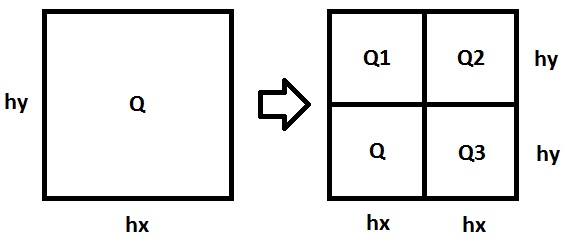
\includegraphics[width=1\textwidth]{Q.jpg} \hspace*{7cm}
     \end{center}
   \end{figure}

   Perceba que um valor de $f(x, y)$ que antes caia em $Q$ (da esquerda) agora pode cair em $Q_1$, $Q_2$ e $Q_3$ e que a distância de $(x, y)$ até o inferior esquerdo deste quadrado é menor do que a distância
   deste mesmo ponto vértice inferior esquerdo de $Q$, diminuindo portanto o valor do erro.

   \pagebreak


  \section{Considerações Finais (e pessoais)}

  \indent\indent Do EP2 para este, resolvi alguns problemas de falta de conhecimento que tinha com o \textit{GNU-Octave} para oferecer um código mais limpo e eficiente. A qualidade do código
  com relação ao último EP está incomparavelmente superior, e desta vez eu estou entregando o EP satisfeito com os resultados obtidos e a qualidade do código. Ainda, este relatório traz informações a respeito
  de \textbf{todo trabalho que foi feito}, sem exceções, e responde todas as perguntas presentes no enunciado do EP3 ao longo das 7 seções.

  Com relação à manipulação de imagens, o problema que eu tive com os índices no EP2 foi aparentemente resolvido neste EP, dado que eu consegui atingir resultados deveras satisfatórios para a interpolação da imagem exemplo.
  Este EP3 não foi feito copiando e colando o EP2 e `melhorando as partes ruins'. Tudo foi replanejado e reimplementado, ora até usando outras estruturas de dados, tal como \textit{Struct Arrays}.

  Ainda, a maneira que eu aproximei as imagens no EP2 não usou nas bordas as expansões de Taylor para 3 pontos para frente, para trás, para cima e para baixo (apenas fazia a média aritmética entre o ponto da borda
  e o \textit{pixel} vizinho conhecido do eixo correspondente), diferentemente do que foi feito neste EP3.

  Finalmente, como o EP3 sugeriu uma idéia de continuidade do EP2 (e pensando em boas práticas de desenvolvimento de \textit{software}), eu resolvi aproveitar a explicação da dedução dos cálculos dos
  coeficientes dos métodos de interpolação nessa documentação apenas porque me pareceu a coisa mais correta a se fazer, mesmo que isso não tivesse sido pedido no enunciado. Com isso a documentação fica, de fato, completa.

\end{document}
